\chapter{(Optional) Diffusion Models and Optimal Transport}\label{ch:ot-eot}



Mapping one distribution to another (with generation as a special case) 
is a central challenge. Flow matching addresses this by learning a 
time-dependent velocity field that transports mass from source to target. 
This naturally connects to transport theory: classical optimal transport 
seeks the minimal cost path between distributions, while its entropy 
regularized form, the Schr\"odinger bridge, selects the most likely 
controlled diffusion relative to a reference such as Brownian motion. 

In this chapter we review the foundations of optimal transport, entropic 
optimal transport, and Schr\"odinger bridges as formulations of the 
distribution–to–distribution problem. This leads to a central question: 
to what extent do diffusion models realize such optimal transports? 
They admit two views: as \emph{stochastic processes}, defined through 
forward and reverse SDEs, and as \emph{deterministic processes}, given 
by PF-ODEs. The stochastic view aligns directly with 
entropic optimal transport, while the PF-ODE does not 
generally correspond to any known transport objective. This gap leaves 
an open question: under what conditions can diffusion models be regarded 
as solving an optimal transport problem?




\newpage
\section{Prologue of Distribution-to-Distribution Translation} 
Diffusion models fix the terminal distribution to a standard Gaussian, $p_{\mathrm{prior}}$.  
However, many applications require \emph{distribution-to-distribution} translation: transforming a source distribution $p_{\mathrm{src}}$ into a different target $p_{\mathrm{tgt}}$.  
Examples include converting sketches to photorealistic images or translating between artistic styles.

Modern diffusion methods provide practical ways to achieve this.  
\emph{One-endpoint} methods such as SDEdit~\citep{meng2021sdedit} begin with a source image at $t=0$, diffuse it to an intermediate step $t$, and then use a pre-trained diffusion model for the target domain to reverse the process.  
This produces an output that matches the style and content of the target distribution.  

\emph{Two-endpoint} methods, like Dual Diffusion Bridge~\citep{su2022dual}, instead connect the two domains through a shared latent distribution, typically a Gaussian at $t=1$.  
A forward probability–flow ODE transports samples from $p_{\mathrm{src}}$ into this latent space, while a reverse ODE trained on the target domain maps them back to $p_{\mathrm{tgt}}$.  
Beyond such sampling-time approaches, the Flow Matching framework described in \Cref{sec:flow-matching-framework} offers a training-based alternative: it directly learns an ODE flow that continuously moves mass from $p_{\mathrm{src}}$ to $p_{\mathrm{tgt}}$.  

Crucially, transforming between distributions requires more than two separately trained models. 
It demands a principled mapping that aligns the dynamics at \emph{both} endpoints and does so in the ``cheapest'' (cost-efficient) way. 

In this section, rather than surveying the many diffusion-based translation applications, we shift our focus to the mathematical foundations of this classic distribution-to-distribution problem.  
In particular, we highlight optimal transport (OT) and its entropic variant, the Schrödinger bridge (SB), which have long been studied in the theoretical community as canonical formulations of cost-efficient (in mathematical sense) distributional transformation.



At its core,  the fundamental question is: 
\begin{question}
    Given two probability distributions, what is the most efficient way to transform one into the other while minimizing the total \emph{cost}?
\end{question}
Here, the cost, $ c(\mathbf{x}, \mathbf{y}) $, is a non-negative function that assigns a penalty for moving a unit of mass from a point $ \mathbf{x}  $ to a point $ \mathbf{y}$. A common choice is the squared distance, $c(\mathbf{x}, \mathbf{y}) = \|\mathbf{x} - \mathbf{y}\|^2$.

This section provides a brief overview to clarify how diffusion-based approaches, including flow matching, connect to classical and regularized optimal transport. The central question we aim to explore is:
\begin{question}
    Is a diffusion model a form of optimal transport connecting $p_{\text{data}}$ and $p_{\text{prior}}$, and in what sense?
\end{question}


To address this question, we first clarify what ``optimality'' means in
\Cref{sec:ot-intro}. We review classical \emph{optimal transport (OT)} in the static
Monge--Kantorovich form (\Cref{eq:ot}) and its dynamic Benamou--Brenier formulation (\Cref{eq:bb-ot}; minimizing
kinetic energy subject to the continuity equation), as well as the entropy
regularized variant (\emph{entropic OT}) in \Cref{eq:eot-epsilon}, which is equivalent to the \emph{Schr\"odinger
Bridge Problem} (\Cref{eq:sb-kinetic}). In the dynamic view, OT induces a deterministic flow
satisfying the continuity equation, whereas SB induces a controlled diffusion
whose marginals evolve by the Fokker-Planck equation. We provide a high level
map between these formulations in \Cref{sec:relation-ot}.

We then split the discussion into two parts. First, in \Cref{sec:dm-and-sb}, we
explain that the fixed forward noising SDE used in standard diffusion models is
not, by itself, a Schr\"odinger bridge between arbitrary $p_{\mathrm{src}}$ and
$p_{\mathrm{tgt}}$: the forward process is a chosen reference diffusion and both forward-in-time or reverse-time SDE do not, in general, enforce exact endpoint matching to a prescribed target. Hence
it is not entropic OT optimal unless  one explicitly solves the SB problem with those
endpoints; while it is an optimal solution to the half-bridge problem as it is anchored with one starting point.

Second, in \Cref{sec:pfode-ot}, we return to the generative setting with
$p_{\mathrm{src}}=p_{\mathrm{prior}}$ (Gaussian) and
$p_{\mathrm{tgt}}=p_{\mathrm{data}}$. The PF-ODE  defines a deterministic map that transports
$p_{\mathrm{prior}}$ to $p_{\mathrm{data}}$ by construction. However, this flow is generally not an OT map for a prescribed transport cost (e.g., quadratic $W_2$): it realizes one admissible deterministic coupling among many and does not minimize the Benamou–Brenier action. What follows is we discuss if the ``rectify flow'' procedure  (\Cref{subsec:rectify}) can lead to a OT map; however, in general, there is no such theoretical guarantee. Therefore, the exact characterization between diffusion model's PF-ODE map and OT remains a challenging and unsolved problem.


\newpage
\section{Taxonomy of the Problem Setups}\label{sec:ot-intro} 
In this section, we introduce notions of what constitutes the most ``efficient'' or ``optimal'' way to transport mass from $p_{\mathrm{src}}$ to $p_{\mathrm{tgt}}$. These include classical optimal transport (OT) and its entropy-regularized variant, which admits an equivalent formulation known as the Schrödinger Bridge. This taxonomy provides background that will later clarify connections with diffusion models.





\subsection{Optimal Transport (OT)}  

\begin{figure}[th!]
    \centering
    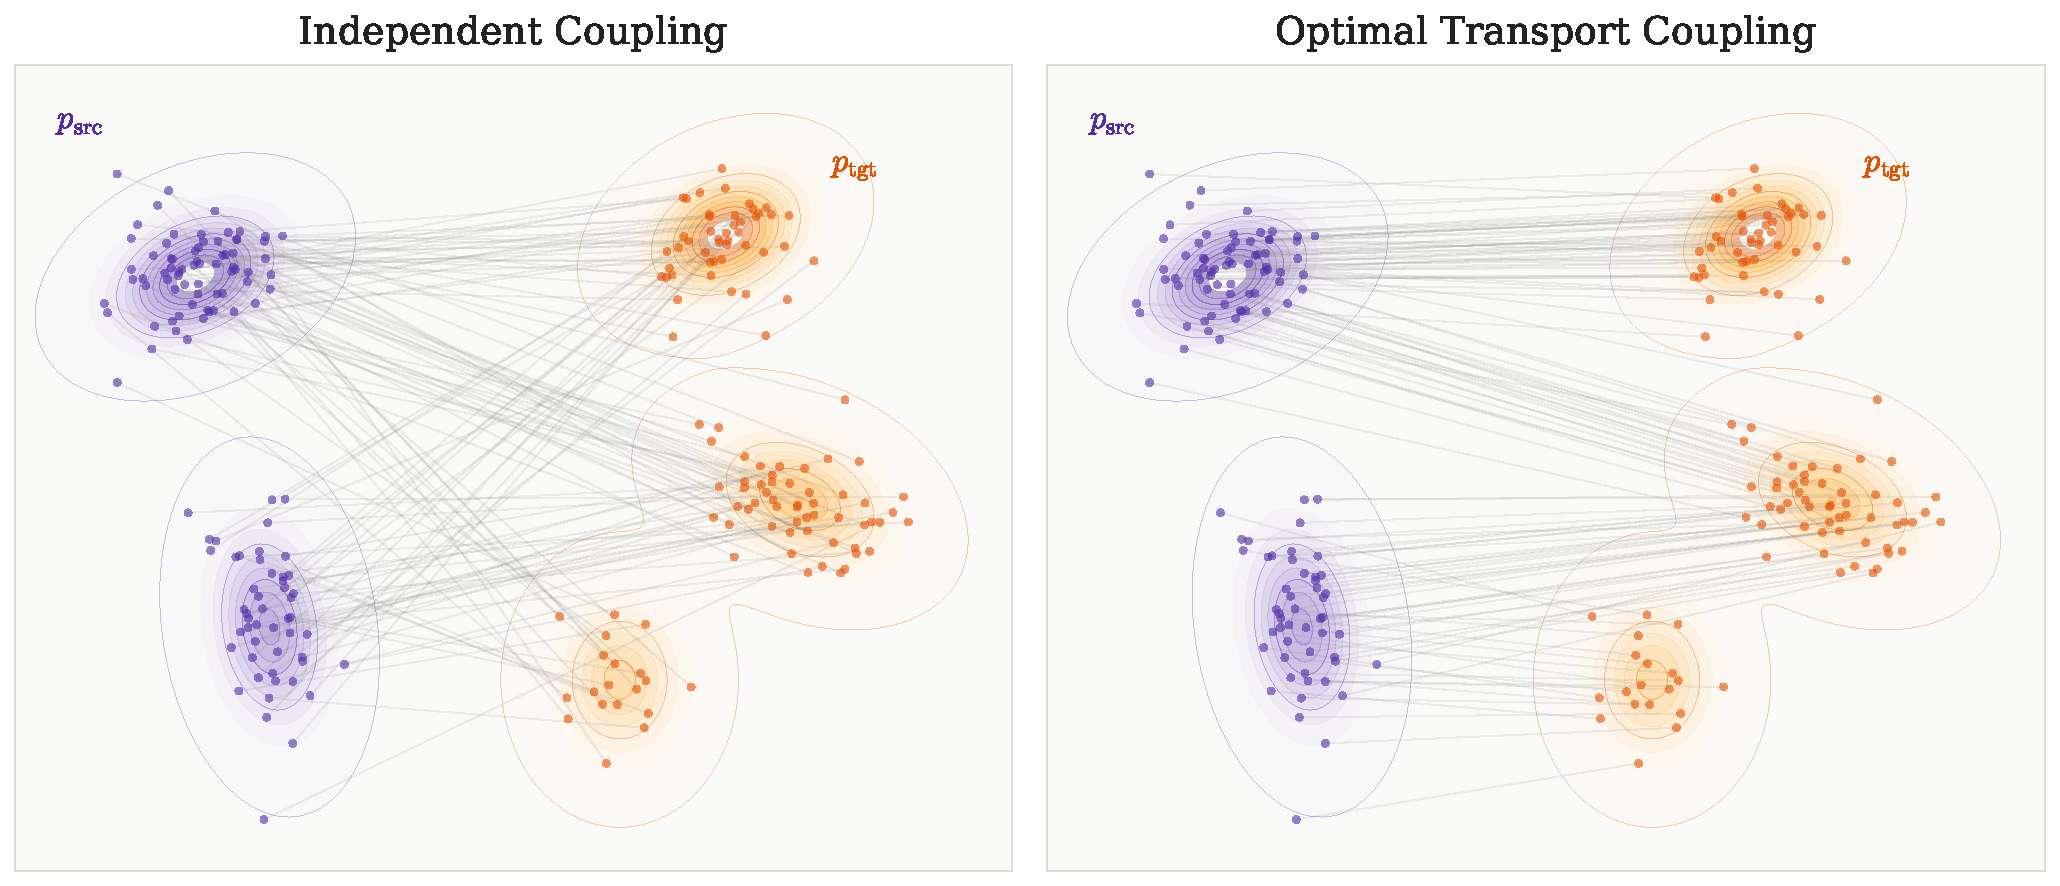
\includegraphics[width=\linewidth]{Images/PartB/ot_2d_coupling_comparison.pdf}
    \caption{\textbfs{Two couplings between the same $p_{\mathrm{src}}$ and $p_{\mathrm{tgt}}$ in 2D.}
    Left: independent (random) pairing produces crossing paths with high cost.
    Right: the optimal transport coupling pairs nearby mass, avoiding crossings.
    \figcredit{Created by the authors with AI-assisted coding.}}
    \label{fig:ot-2d-coupling}
\end{figure}

\paragraph{Monge--Kantorovich (Static) Formulation of OT Problem.}
We fix a cost function $c:\R^D\times\R^D\to\R$ that specifies the expense of sending probability mass
from $\rvx$ to $\rvy$. The goal is to transform the source distribution $p_{\mathrm{src}}$ into the target
distribution $p_{\mathrm{tgt}}$ as cheaply as possible.

To even define a cost, we must know which pairs $(\rvx,\rvy)$ are matched. This role is played by a
\emph{coupling}: a joint distribution $\gamma$ on $\R^D\times\R^D$ whose marginals are
$p_{\mathrm{src}}$ and $p_{\mathrm{tgt}}$. In other words, sampling $(\rvx,\rvy)\sim\gamma$ means we match
$\rvx$ from the source with $\rvy$ from the target. If $\gamma$ admits a density $\gamma(\rvx,\rvy)$ with
respect to Lebesgue measure, the marginal constraints read
\[
\int_{\R^D} \gamma(\rvx,\rvy)\,\diff \rvy = p_{\mathrm{src}}(\rvx), 
\qquad 
\int_{\R^D} \gamma(\rvx,\rvy)\,\diff \rvx = p_{\mathrm{tgt}}(\rvy).
\]
That is, integrating out $\rvy$ recovers the source density in $\rvx$, while integrating out $\rvx$
recovers the target density in $\rvy$.

We give two standard examples for illustration:
\begin{enumerate}
    \item \textbfs{Discrete Supports.}  
    If $p_{\mathrm{src}}$ and $p_{\mathrm{tgt}}$ are supported on finitely many points, a coupling is
    represented by a nonnegative matrix $(\gamma_{ij})$ whose row sums equal $p_{\mathrm{src}}(i)$ and
    column sums equal $p_{\mathrm{tgt}}(j)$. Each entry $\gamma_{ij}$ is the amount of mass sent from
    $i$ to $j$.
    \item \textbfs{Deterministic Map.}  
    If there exists a measurable map $\rmT$ with $\rmT_\#p_{\mathrm{src}}=p_{\mathrm{tgt}}$, then
    $\gamma=(\rmI,\rmT)_\#p_{\mathrm{src}}$ is a deterministic coupling that moves each point
    $\rvx$ directly to $\rmT(\rvx)$.
\end{enumerate}

Once a coupling $\gamma$ is fixed, the transport cost is simply the average unit cost under this plan:
\[
\int c(\rvx,\rvy)\,\diff\gamma(\rvx,\rvy)
=\E_{(\rvx,\rvy)\sim\gamma}\!\big[c(\rvx,\rvy)\big].
\]
In the discrete case, this reduces to $\sum_{i,j} c_{ij}\gamma_{ij}$, whereas in
the continuous setting it becomes a double integral. In what follows, we will
focus only on the continuous case.

The optimal transport problem is then to choose, among all admissible couplings,
the one that minimizes this expected cost.
\begin{mdframed}
\begin{equation}\label{eq:ot}
\mathrm{OT}\big(p_{\mathrm{src}},p_{\mathrm{tgt}}\big)
:= \inf_{\gamma\in\Gamma(p_{\mathrm{src}},p_{\mathrm{tgt}})}
\int c(\rvx,\rvy)\,\diff\gamma(\rvx,\rvy),
\end{equation}
\end{mdframed}
where the feasible set simply enforces the marginal, or mass-conservation, constraints:
\begin{align*}
    \Gamma(p_{\mathrm{src}},p_{\mathrm{tgt}})
= \Big\{\gamma \in &\mathcal{P}(\R^D\times\R^D): \\
&\int \gamma(\rvx,\rvy) \diff \rvy = p_{\mathrm{src}}(\rvx),\,\,
\int \gamma(\rvx,\rvy)\diff \rvx = p_{\mathrm{tgt}}(\rvy)\Big\},
\end{align*}
where $\mathcal{P}(\R^D\times\R^D)$ denotes the set of all probability measures on
$\R^D\times\R^D$.  


\subparagraph{A Special Case: Wasserstein-2 Distance.}

The Wasserstein-2 distance  is a special case of the Monge--Kantorovich problem with the quadratic cost $c(\mathbf{x}, \mathbf{y}) = \|\mathbf{x} - \mathbf{y}\|^2$. It measures the distance between two probability distributions as follows:
\begin{align*}
 \mathcal{W}_2^2(p_{\mathrm{src}}, p_{\mathrm{tgt}}) := \inf_{\gamma \in \Gamma(p_{\mathrm{src}}, p_{\mathrm{tgt}})} \mathbb{E}_{(\mathbf{x}, \mathbf{y}) \sim \gamma} \left[ \|\mathbf{x} - \mathbf{y}\|^2 \right].
\end{align*}

Under suitable assumptions on $p_{\mathrm{src}}$ and $p_{\mathrm{tgt}}$, Brenier's theorem (see \Cref{thm:brenier})\footnote{Brenier's theorem is about the existence and structure of the optimal transport map for quadratic cost. In particular, if $p_{\mathrm{src}}$ does not give mass to sets of dimension at most $D-1$, then an optimal transport map $\rmT^*$ uniquely exists.} guarantees that the optimal coupling $\gamma$ for the quadratic cost is concentrated on the graph of a deterministic map $\rmT:\mathbb{R}^D \rightarrow \mathbb{R}^D$. Consequently, the Wasserstein-2 distance can be equivalently expressed as\footnote{There are three commonly used formulations of the $\mathcal{W}_2$ distance: the Monge formulation (based on an optimal transport map), the Kantorovich formulation (based on couplings), and the Benamou--Brenier dynamic formulation (see \Cref{eq:bb-ot}). These are equivalent under appropriate regularity conditions.}:
\begin{equation}\label{eq: Monge's Formulation}    \mathcal{W}_2^2(p_{\mathrm{src}}, p_{\mathrm{tgt}}) = \inf_{\substack{\rmT:\mathbb{R}^D \rightarrow \mathbb{R}^D,\\ \text{ s.t. }\rmT\#p_{\mathrm{src}} = p_{\mathrm{tgt}}}} \mathbb{E}_{\rvx \sim p_{\mathrm{src}}} \left[ \| \rmT(\rvx) - \rvx \|^2 \right].
\end{equation}
Here, $\rmT\#p_{\mathrm{src}} = p_{\mathrm{tgt}}$ means that $ \rmT $ pushes $ p_{\mathrm{src}} $ forward to $ p_{\mathrm{tgt}} $, i.e., $ \rmT(\rvx) \sim p_{\mathrm{tgt}} $ for $ \rvx \sim p_{\mathrm{src}}$. 

 

Thus, the Wasserstein-2 distance represents the minimal expected squared transport cost among all couplings or transport maps that match the given marginals. The optimal transport map denoted by $\rmT^*(\mathbf{x})$, known as the \emph{Monge map}, yields the most efficient way to transform $p_{\mathrm{src}}$ into $p_{\mathrm{tgt}}$.

\paragraph{Benamou--Brenier (Dynamic) Formulation of OT.} 
\begin{figure}[th!]
    \centering
    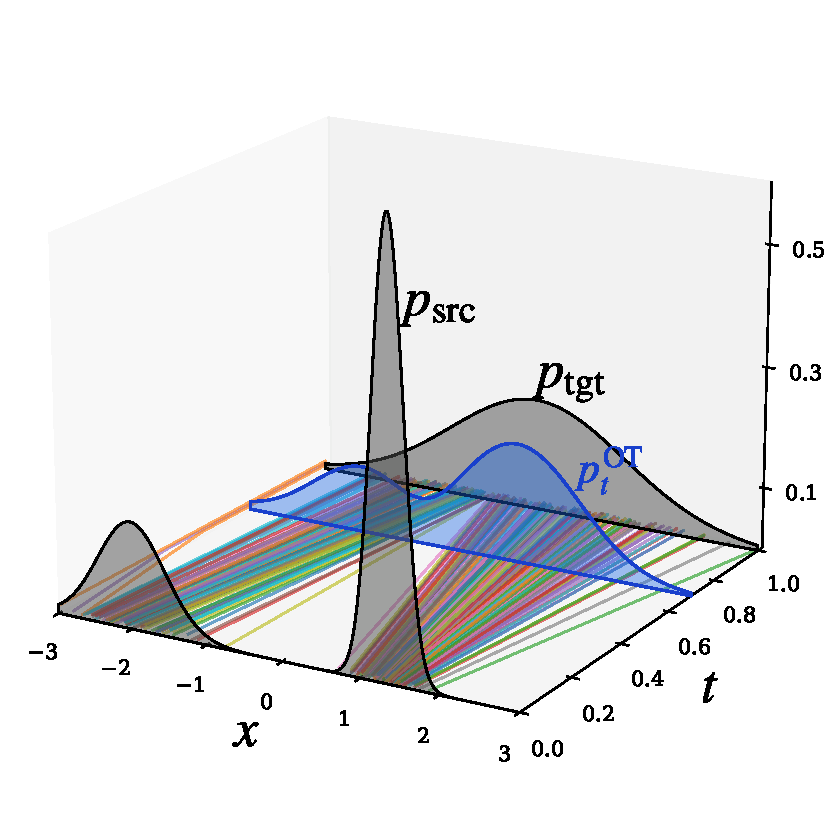
\includegraphics[width=0.8\linewidth]{Images/PartB/ot_illustration.pdf}
    \caption{ \textbfs{Illustration of dynamic view of OT.} The interpolation $p_t^{\mathrm{OT}}$ evolves continuously in time, 
providing the least-cost transport plan that deterministically maps 
$p_{\mathrm{src}}$ to $p_{\mathrm{tgt}}$ (the McCann's displacement interpolation).
\figcredit{Created by the authors.}}
    \label{fig:ill-ot}
\end{figure}



Instead of mapping distributions directly in a static manner, as in the Monge--Kantorovich formulation, transport can also be modeled as a continuous-time flow:
\begin{equation*}
    p_0 := p_{\mathrm{src}} \to p_t \to p_1 := p_{\mathrm{tgt}}, \quad t \in [0,1].
\end{equation*}
This dynamic formulation of optimal transport, introduced by \citet{benamou2000computational}, seeks a smooth velocity field $ \rvv_t(\rvx) $ that describes how mass in $ p_t(\rvx) $ evolves over time.

The Benamou--Brenier formulation\footnote{Benamou–Brenier formulation describes how to compute the $ \mathcal{W}_2 $ distance by minimizing kinetic energy over continuous paths of measures and velocities.} shows that, for the quadratic cost $ c(\rvx, \rvy) = \|\rvx - \rvy\|_2^2 $ (i.e., the $ \mathcal{W}_2 $ distance), the optimal value of the static OT problem in \Cref{eq:ot} is equal to the optimal value of the kinetic energy minimization problem:
%the static OT problem in \Cref{eq:ot} is equivalent \doh{``Equivalent'' is unclear.} to the following dynamic formulation:
\begin{mdframed}
   \begin{equation}\label{eq:bb-ot}
    \mathcal{W}_2^2(p_{\mathrm{src}}, p_{\mathrm{tgt}}) = \min_{\substack{ (p_t, \rvv_t) \text{ s.t. }
        \partial_t p_t + \nabla \cdot (p_t \rvv_t) = 0, \\
        p_0 = p_{\mathrm{src}},\,\, p_1 = p_{\mathrm{tgt}}
    }}
    \int_0^1 \int_{\mathbb{R}^D} \|\rvv_t(\rvx)\|^2 p_t(\rvx) \diff\rvx \diff t
\end{equation} 
\end{mdframed}
where $p_t$ is a probability distribution on $\mathbb{R}^D$ for each $t \in [0,1]$. In particular, The optimal transport flow $p_t(\rvx)$ follows \textit{McCann’s displacement interpolation}:
\begin{equation*}
    \rmT_t^*(\rvx) = (1 - t)\rvx + t\rmT^*(\rvx),
\end{equation*}
where $\rmT^*(\rvx)$ is the OT map that transports $p_{\mathrm{src}}$ to $p_{\mathrm{tgt}}$. This linear interpolation moves mass along straight lines with constant velocity: $p_t = \rmT_t^*\#p_{\mathrm{src}}$ for each $t \in [0,1]$. 

The optimal transport map $\rmT^*$ satisfies the \emph{Monge–Ampère equation}:
%However, computing $\rmT^*$ generally requires solving the \emph{Monge–Ampère equation}:
\begin{equation}\label{eq:monge-ampere}
    p_{\mathrm{tgt}}\left(\nabla \psi(\rvx)\right) \det\left(\nabla^2 \psi(\rvx)\right) = p_{\mathrm{src}}(\rvx),
\end{equation}
where $\rmT^*(\rvx) = \nabla \psi(\rvx)$ for some convex function $\bpsi$ by Brenier’s theorem. However, this nonlinear PDE is typically intractable for explicit solutions. Note that this is precisely the change-of-variables relation used by normalizing flows (c.f., \Cref{eq:nf-change-of-var}): flows parametrize an invertible transport map with a tractable Jacobian determinant, but do not in general impose the gradient-of-potential structure $\rmT^*=\nabla\psi$; consequently, a trained flow can differ substantially from the Brenier/OT map.





\subsection{Entropy-Regularized Optimal Transport (EOT)}

To motivate EOT concretely, consider empirical distributions built from samples. 
Suppose $p_{\mathrm{src}}$ is supported on points $\{\rvx^{(i)}\}_{i=1}^n \subset \R^D$ with weights $a_i$, 
and $p_{\mathrm{tgt}}$ on $\{\rvy^{(j)}\}_{j=1}^n \subset \R^D$ with weights $b_j$. 
A coupling is then an $n\times n$ nonnegative matrix $\gamma=(\gamma_{ij})$ whose row sums match $a$ and column sums match $b$. 
Each entry $\gamma_{ij}$ represents the amount of mass transported from $\rvx^{(i)}$ to $\rvy^{(j)}$\footnote{Empirical (discrete) measures provide a principled proxy for continuous distributions. 
When the ground cost is $c(x,y)=d(x,y)^p$ (so the OT value equals $W_p^p$) and the measures have finite $p$th moments, the empirical measures converge to the population in $W_p$ with quantitative rates; see \citet{fournier2015rate} and the overview in \citet{peyre2019computational}.}.

\paragraph{Why Regularize OT?}
Classical OT in this discrete setting (obtained by taking counting measures in the continuous formulation \Cref{eq:ot}) reduces to minimizing
\[
\min_{\gamma=(\gamma_{ij})}\sum_{i,j} C_{ij}\,\gamma_{ij},
\]
over all feasible couplings $\gamma=(\gamma_{ij})$, 
where $C_{ij} = c(\rvx^{(i)},\rvy^{(j)})$ is the cost of moving one unit of mass from source point $\rvx^{(i)}$ to target point $\rvy^{(j)}$, for a prescribed ground cost 
$c:\R^D\times\R^D\to\R_{\ge 0}$ (e.g., $c(\rvx,\rvy)=\|\rvx-\rvy\|_2^2$).

Two main issues arise:
\begin{enumerate}
    \item \textbfs{Non-Uniqueness and Instability:} The minimizer $\gamma^*$ need not be unique. 
    For example, if two transport plans achieve the same minimum cost, the solver may select either one. 
    Consequently, small changes in the inputs $(a,b,C)$ (such as moving a sample, adjusting weights, or slightly perturbing costs) can cause abrupt jumps in the solution.  
    \item \textbfs{High Computational Cost:} The problem is a linear program with $n^2$ variables and $2n$ constraints. 
    Practical solvers (e.g., Hungarian algorithm~\citep{kuhn1955hungarian,munkres1957algorithms}, network simplex~\citep{peyre2019computational}) typically scale as $\mathcal{O}(n^3)$, which is infeasible for large $n$.
\end{enumerate}

To overcome these bottlenecks,  EOT objective function introduces a regularization term to the classical OT problem, controlled by a parameter $\varepsilon > 0$:
\begin{mdframed}
    \begin{align}\label{eq:eot-epsilon}
\begin{aligned}
        \text{EOT}_\varepsilon(p_{\mathrm{src}}, p_{\mathrm{tgt}}) &:= \min_{\gamma \in \Gamma(p_{\mathrm{src}}, p_{\mathrm{tgt}})} \int c(\rvx,  \rvy)  \diff\gamma(\rvx, \rvy) 
        + \varepsilon \mathcal{D}_{\text{KL}}\left(\gamma \Vert M \right).
\end{aligned}
\end{align}
\end{mdframed}
The reference measure $M$ is typically chosen as the product of the marginals, $p_{\mathrm{src}} \otimes p_{\mathrm{tgt}}$. The KL divergence term is directly related to the Shannon entropy of the transport plan $\gamma$:
\[
\mathcal{D}_{\text{KL}}(\gamma \,\Vert\, p_{\mathrm{src}} \otimes p_{\mathrm{tgt}}) = -\mathcal{H}(\gamma) + \text{Constant},
\]
where $\mathcal{H}(\gamma) := -\int \gamma(\rvx, \rvy) \log \gamma(\rvx, \rvy) \diff \rvx \diff \rvy$.



The addition of this regularization term yields several theoretical and practical advantages, which we briefly outline below:
\paragraph{Why Entropy Regularizer Helps?}
\begin{enumerate}
  \item \textbfs{Mass Spreading.}
  Since $t\mapsto t\log t$ is convex and grows rapidly for large $t$, minimizing $\int \gamma\log\gamma$
  penalizes \emph{peaky} couplings (some $\gamma(\rvx,\rvy)$ very large, most near zero).
  For fixed total mass $\int \gamma=1$, it favors plans where $\gamma(\rvx,\rvy)$ is more evenly distributed
  over $(\rvx,\rvy)\in\mathbb{R}^D\times\mathbb{R}^D$.
  Equivalently, maximizing Shannon entropy promotes higher ``uncertainty'' (diffuseness).

  \item \textbfs{Strict Convexity and Uniqueness.}
  Because $\mathcal{H}$ is strictly concave, the objective in \Cref{eq:eot-epsilon} is strictly convex in $\gamma$,
  yielding a \emph{unique} minimizer $\gamma^*_\varepsilon$ that depends continuously on $(p_{\mathrm{src}},p_{\mathrm{tgt}},c)$.

  \item \textbfs{Sinkhorn Form and Positivity.}
  Under mild conditions\footnote{We assume that $c<\infty$ holds $p_{\mathrm{src}}\otimes p_{\mathrm{tgt}}$-almost everywhere, and that the marginal kernel integrals are finite and positive. 
For simplicity, we focus on the case where $\gamma^*_\varepsilon$, $p_{\mathrm{src}}$, and $p_{\mathrm{tgt}}$ admit densities with respect to the Lebesgue measure.
},
  the optimizer has the \emph{Schrödinger/Sinkhorn form}
  \[
  \gamma^*_\varepsilon(\rvx,\rvy) = u(\rvx)\, \exp \bigl(-\tfrac{c(\rvx,\rvy)}{\varepsilon}\bigr)  \,v(\rvy)p_{\mathrm{src}}(\rvx) p_{\mathrm{tgt}}(\rvy),
  \]
  for positive scaling functions $u,v$ (unique up to a global factor). In practice, the continuous formulation is approximated with finite samples, reducing EOT to a finite (sampled) Sinkhorn iteration. 
The entropic objective is strictly convex, and the scaling (Sinkhorn/IPFP) algorithm solves it efficiently~\citep{sinkhorn1964relationship,cuturi2013sinkhorn}. 
For a dense problem with $n$ support points per marginal (an $n\times n$ kernel), each Sinkhorn iteration costs $\mathcal{O}(n^2)$ time and $\mathcal{O}(n^2)$ memory, 
making the method more scalable and practical~\citep{altschuler2017near}.

  \item \textbfs{Limits in $\varepsilon$.}
As $\varepsilon \to 0$, the optimal plan $\gamma^*_\varepsilon$ becomes increasingly concentrated, approaching a (possibly singular) classical OT coupling (we will revisit this connection in \Cref{subsec:eot-ot}). 
As $\varepsilon$ increases, $\gamma^*_\varepsilon$ gradually spreads out and approaches the independent coupling $p_{\mathrm{src}}\otimes p_{\mathrm{tgt}}$. 
\end{enumerate}



\subsection{Schrödinger Bridge (SB)}\label{subsec:sb}


\paragraph{KL Formulation of SB.}
The Schrödinger Bridge (SB) problem, introduced by Erwin Schrödinger in the 1930s,
asks the following question. Suppose particles move according to some simple
reference dynamics, such as Brownian motion. Now imagine that we observe the
particles at two times: at $t=0$ their distribution is $p_{\mathrm{src}}$, and
at $t=1$ it is $p_{\mathrm{tgt}}$. Among all possible stochastic processes
that connect these two distributions, which one deviates the least from the
reference dynamics? Here ``deviation'' is measured by the KL divergence, so the
solution to the SB problem is the most likely way to deform Brownian motion
into a process that satisfies the prescribed boundary conditions.

To make this precise, let $\rvx_{0:T}:=\{\rvx_t\}_{t\in[0,T]}$ denote a complete
trajectory of the process. We write $P$ for the \emph{law of trajectories},
that is, the probability distribution over entire sample paths. The time-$t$
marginal of $P$ is denoted by $p_t$ (or $P_t$), which describes the
distribution of the state $\rvx_t$ at a single time. Formally, for a measurable
set $A\subseteq\mathbb R^D$,
\[
p_t(A) = P(\rvx_t \in A).
\]
In other words, $p_t$ can be viewed as the empirical distribution obtained by
sampling many full trajectories from $P$ and then collecting the states at
time $t$—for instance, as a histogram if the state is one-dimensional.


Consider a reference diffusion $\{\rvx_t\}_{t\in[0,T]}$ governed by the SDE
\begin{align}\label{eq:general-sb-sde}
    \diff \rvx_t  =  \rvf(\rvx_t,t)\,\diff t  +  g(t)\,\diff \rvw_t,
\end{align}
where $\rvf\colon \R^D\times[0,T]\!\to\!\R^D$, $g\colon[0,T]\!\to\!\R$, and
$\{\rvw_t\}_{t\in[0,T]}$ is a standard Brownian motion.  
Let $R$ denote the \emph{path law} (joint distribution) of the full trajectory
$\rvx_{0:T}:=\{\rvx_t\}_{t\in[0,T]}$; this $R$ will serve as the \emph{reference}
trajectory distribution.

With this notation, the SB problem seeks a trajectory law $P$
that is closest to $R$ in KL divergence while matching the prescribed endpoint
marginals:
\begin{align}\label{eq:sb-epsilon-general}
    \mathrm{SB}(p_{\mathrm{src}}, p_{\mathrm{tgt}})
    := \min_{P}\, \mathcal{D}_{\mathrm{KL}}(P\|R)
    \quad \text{s.t.} \quad P_0 = p_{\mathrm{src}},\;\; P_T = p_{\mathrm{tgt}}.
\end{align}
The optimizer $P^*$ depends on the chosen reference process $R$.

\paragraph{Stochastic control view of SB.}

\begin{figure}[th!]
    \centering
    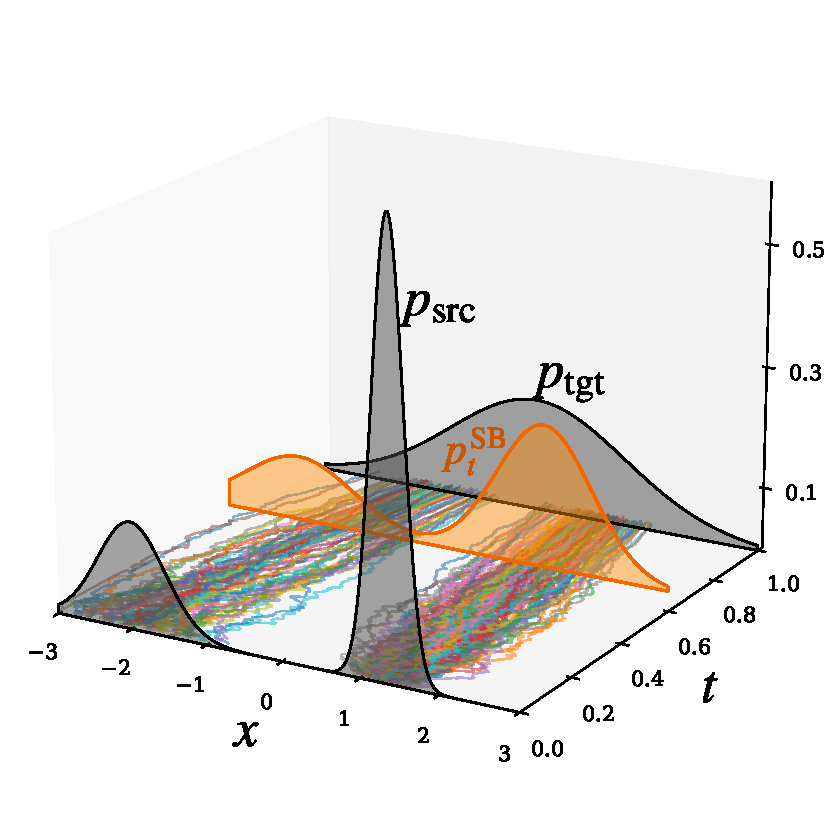
\includegraphics[width=0.8\linewidth]{Images/PartB/sb_illustration.pdf}
    \caption{\textbfs{Illustration of stochastic control view of SB.} The bridge seeks the stochastic path that deviates least from the reference while connecting $p_{\mathrm{src}}$ and $p_{\mathrm{tgt}}$.
    \figcredit{Created by the authors.}}
    \label{fig:ill-sb}
\end{figure}


Rather than optimizing over arbitrary path distributions $P$ in
\Cref{eq:sb-epsilon-general}, a more tractable approach is to take the reference
dynamics as an anchor and allow it to drift. This is done by
introducing a time-dependent drift $\rvv_t(\rvx_t)$, which perturbs the
reference process and generates a family of candidate trajectory
distributions. The resulting dynamics take the form of a \emph{controlled
diffusion}:
\[
    \diff \rvx_t
    = \bigl[\rvf(\rvx_t,t) + \rvv_t(\rvx_t)\bigr]\diff t + g(t) \diff \rvw_t,
\]
where $\rvv_t:\R^D\to\R^D$ is the drift to be optimized later (\Cref{eq:sb-kinetic}).
 Under standard integrability
conditions (e.g., Novikov’s condition) and by Girsanov’s theorem
(see \Cref{subsec:girsanov}), the KL divergence between the controlled law $P$
and the reference $R$ admits the dynamic (kinetic) form
\begin{align*}
    \mathcal{D}_{\mathrm{KL}}(P\|R)
    = \E_{P}\!\left[\frac{1}{2}\int_0^T \frac{\|\rvv_t(\rvx_t)\|^2}{g^2(t)} \diff t\right]
    = \frac{1}{2}\int_0^T\!\int_{\R^D}\frac{\|\rvv_t(\rvx)\|^2}{g^2(t)} p_t(\rvx) \diff \rvx \diff t,
\end{align*}
where $p_t$ is the time–$t$ marginal of $\rvx_t$ under the controlled process. The
second equality follows from the law of total expectation.

Hence, the SB problem can be reformulated as minimizing the expected control
energy over all admissible drifts $\rvv_t$ that steer the process from
$p_{\mathrm{src}}$ at $t=0$ to $p_{\mathrm{tgt}}$ at $t=T$
\citep{dai1991stochastic,pra1990markov,pavon1991free,chen2016relation}.
This leads to the \emph{stochastic control formulation}:
\begin{mdframed} 
\begin{align}\label{eq:sb-kinetic} 
\begin{aligned} &\mathrm{SB}_\varepsilon(p_{\mathrm{src}}, p_{\mathrm{tgt}}) \\= & \min_{\substack{ \mathbf{v}_t \text{ s.t. } \diff \rvx_t = \left[\rvf(\rvx_t, t) + \mathbf{v}_t(\rvx_t) \right]\diff t + g(t) \diff \rvw_t, \\ \rvx_0 \sim p_{\mathrm{src}}, \,\, \rvx_T \sim p_{\mathrm{tgt}} }} \frac{1}{2} \int_0^T\int_{\mathbb{R}^D} \frac{\norm{\rvv_t(\rvx)}^2}{g^2(t)} p_t(\rvx)\diff \rvx \diff t, 
\end{aligned}
\end{align} 
\end{mdframed}

Importantly, the endpoint distributions $p_{\mathrm{src}}$ and $p_{\mathrm{tgt}}$ are arbitrary;
the control $\rvv_t$ is chosen precisely to ``bridge'' the reference dynamics between
these marginals while staying as close as possible (in KL divergence) to the reference
process $R$.

\paragraph{A Special Brownian Reference.}
\Cref{eq:sb-kinetic} resembles the Benamou--Brenier formulation of OT
in \Cref{eq:bb-ot}, especially when the reference process
$R^\varepsilon$ (with $\varepsilon>0$) is chosen to be a Brownian
motion\footnote{This resemblance can be made precise. In an equivalent
time-symmetric fluid-dynamic formulation, if $\tilde{\rvv}_t$ denotes
the current velocity satisfying the continuity equation
$\partial_t \rho_t + \nabla \cdot (\rho_t \tilde{\rvv}_t)=0$, then the
Brownian-reference SB objective (\Cref{eq:sb-epsilon-kinetic}) can be
written as a Benamou--Brenier-type kinetic term, up to a conventional
constant factor, plus a Fisher information term:
\[
\int_0^T\!\!\int
\left[
\frac{1}{2}\|\tilde{\rvv}_t(\rvx)\|^2
+
\frac{\varepsilon^2}{8}\|\nabla_{\rvx}\log \rho_t(\rvx)\|^2
\right]\rho_t(\rvx)\,\diff\rvx\,\diff t.
\]
Thus, in the Brownian-reference / quadratic-cost case, entropic OT can
be viewed as a Fisher-information-regularized version of dynamic OT; see
Problem~4.6 in~\citet{chen2021stochastic}.}:
\[
\diff \rvx_t = \sqrt{\varepsilon}\,\diff\rvw_t,
\]
so that $\rvf \equiv \mathbf{0}$ and $g(t) \equiv \sqrt{\varepsilon}$.

In this setting, the SB problem seeks a path distribution $P$ that stays closest
(in KL divergence) to the Brownian reference $R^\varepsilon$, while matching the
endpoint marginals:
\begin{align}\label{eq:sb-epsilon}
    \mathrm{SB}_\varepsilon(p_{\mathrm{src}}, p_{\mathrm{tgt}})
    := \min_{P} \mathcal{D}_{\mathrm{KL}}(P \| R^\varepsilon)
    \quad \text{s.t.} \quad P_0 = p_{\mathrm{src}}, \;\; P_T = p_{\mathrm{tgt}}.
\end{align}
The equivalent stochastic control formulation then becomes
\begin{align}\label{eq:sb-epsilon-kinetic}
\begin{aligned}
    \mathrm{SB}_\varepsilon(p_{\mathrm{src}}, p_{\mathrm{tgt}})
    = \min_{\substack{
        \rvv_t \text{ s.t. } \diff \rvx_t = \rvv_t(\rvx_t)\,\diff t + \sqrt{\varepsilon}\,\diff \rvw_t, \\
        \rvx_0 \sim p_{\mathrm{src}},\;\; \rvx_T \sim p_{\mathrm{tgt}}
    }}
    \frac{1}{2\varepsilon}\int_0^T \!\!\int_{\R^D}
        \|\rvv_t(\rvx)\|^2 \, p_t(\rvx)\,\diff \rvx\,\diff t,
\end{aligned}
\end{align}
where $p_t$ denotes the time--$t$ marginal of diffusion driven by the drift $\rvv_t$:
\[
\diff \rvx_t = \rvv_t(\rvx_t)\,\diff t + \sqrt{\varepsilon}\,\diff \rvw_t.
\]



\paragraph{Why We Need to Specify a Reference Distribution?} 
Unlike in classical OT, the SB problem requires a reference distribution due to its stochastic nature. In OT, the cost function (e.g., $c(\rvx, \rvy) \propto \|\rvx - \rvy\|^2$) implicitly defines a unique, deterministic geodesic path, making a reference unnecessary. In contrast, the SB setting admits infinitely many stochastic processes connecting the marginals, with no intrinsic notion of a ``natural'' path. The reference measure $R$ encodes the system's underlying physics or geometric structure (e.g., Brownian motion) and defines the KL-based optimization objective $\mathcal{D}_{\mathrm{KL}}(P \| R)$, without which the notion of optimality is undefined.



\paragraph{Coupled PDE Characterization.}  
A convenient way to describe the SB solution is through two 
space–time potentials $\Psi(x,t)$ and $\widehat{\Psi}(x,t)$. Let
$p_t^{\mathrm{SB}}$ denote the marginal at time $t\in[0,T]$ of the optimal
trajectory law $P^*$ in \Cref{eq:sb-epsilon-general}. Then one has the
symmetric factorization~\citep{dai1991stochastic}
\begin{align}\label{eq:sb-symmetry}
p_t^{\mathrm{SB}}(x) = \Psi(x,t) \widehat{\Psi}(x,t),
\end{align}
where $\Psi$ and $\widehat{\Psi}$ solve the (linear) \emph{Schrödinger system}~\citep{caluya2021wasserstein,chen2021stochastic,chenlikelihood}:
\begin{align}
\begin{aligned}\label{eq:pde-schrodinger}
\frac{\partial \Psi}{\partial t}(\mathbf{x},t)
  &= -\nabla_{\mathbf{x}} \Psi(\mathbf{x},t) \cdot \rvf(\mathbf{x},t)
     - \frac{g^2(t)}{2}\,\Delta_\mathbf{x} \Psi(\mathbf{x},t),  \\
\frac{\partial \widehat{\Psi}}{\partial t}(\mathbf{x},t)
  &= -\nabla_{\mathbf{x}}\!\cdot\!\bigl(\widehat{\Psi}(\mathbf{x},t)\,\rvf(\mathbf{x},t)\bigr)
     + \frac{g^2(t)}{2}\,\Delta_\mathbf{x}\widehat{\Psi}(\mathbf{x},t) 
\\[4pt] \text{subject to}  \\[4pt]
\Psi(\mathbf{x},0)&\,\widehat{\Psi}(\mathbf{x},0) = p_{\mathrm{src}}(\mathbf{x}),
\quad
\Psi(\mathbf{x},T)\,\widehat{\Psi}(\mathbf{x},T) = p_{\mathrm{tgt}}(\mathbf{x}). 
\end{aligned}
\end{align}

\iffalse

\begin{align}
\begin{aligned}\label{eq:pde-schrodinger}
\frac{\partial \Psi}{\partial t}(\mathbf{x},t)
  &= -\nabla_{\mathbf{x}} \Psi(\mathbf{x},t)^\top\,\rvf(\mathbf{x},t)
     - \frac{1}{2}\,\mathrm{Tr}\bigl(g^2(t)\,\nabla_{\mathbf{x}}^2\Psi(\mathbf{x},t)\bigr),  \\
\frac{\partial \widehat{\Psi}}{\partial t}(\mathbf{x},t)
  &= -\nabla_{\mathbf{x}}\!\cdot\!\bigl(\widehat{\Psi}(\mathbf{x},t) \rvf(\mathbf{x},t)\bigr)
     + \frac{1}{2} \mathrm{Tr}\bigl(g^2(t)\,\nabla_{\mathbf{x}}^2\widehat{\Psi}(\mathbf{x},t)\bigr) 
\\[4pt] \text{subject to}  \\[4pt]
\Psi(\mathbf{x},0)& \widehat{\Psi}(\mathbf{x},0) = p_{\mathrm{src}}(\mathbf{x}),
\quad
\Psi(\mathbf{x},T) \widehat{\Psi}(\mathbf{x},T) = p_{\mathrm{tgt}}(\mathbf{x}). 
\end{aligned}
\end{align}
\fi

\subparagraph{Forward-Time Schrödinger Bridge SDE.}
Once $\Psi$ is known, the optimal dynamics is the reference diffusion tilted by
the space–time factor $\Psi$:
\begin{align}\label{eq:sb-forward-sde}
    \diff \rvx_t = \bigl[\rvf(\rvx_t, t) + g^2(t)\,\nabla_{\mathbf{x}} \log \Psi(\rvx_t, t)\bigr]\diff t
+ g(t)\diff \rvw_t, \quad \rvx_0 \sim p_{\mathrm{src}}.
\end{align}
Let $Q$ denote the trajectory law of \Cref{eq:sb-forward-sde}
(so $Q_0=p_{\mathrm{src}}$ and $Q_T=p_{\mathrm{tgt}}$ by
\Cref{eq:sb-symmetry,eq:pde-schrodinger}). Then
\emph{$Q=P^*$} and the minimizer $\rvv^*$ to \Cref{eq:sb-kinetic} is (see \citep{chen2021stochastic}'s Section 4.6): 
\[
\rvv_t^{*}(\rvx) = g^2(t) \nabla_\rvx \log \Psi(\rvx,t).
\]
That is,
drift correction $g^2\nabla_\rvx\log\Psi$ is precisely the
minimal KL perturbation of the reference needed to match the endpoint
marginals. 

%\textcolor{red}{In other words, the optimal control $\mathbf{v}_t(\rvx_t)$ of the stochastic control formulation \Cref{eq:sb-kinetic} of SB is given by
%\begin{align*}
%    \mathbf{v}_t(\rvx_t) = \rvf(\rvx_t, t) + g^2(t)\,\nabla_{\mathbf{x}} \log \Psi(\rvx_t, t).
%\end{align*}
%}

\subparagraph{Reverse-Time Schrödinger Bridge SDE.}
The same optimal path law can be generated reverse in time. A convenient way
to see the form of the reverse-time drift is to conceptually use the standard time-reversal identity for diffusions:
\[
\rvb^{-}(\rvx,t)=\rvb^{+}(\rvx,t)-g^2(t)\nabla_\rvx\log p_t^{\mathrm{SB}}(\rvx),
\]
where $\rvb^{+}=\rvf+g^2\nabla\log\Psi$ and $p_t=\Psi\,\widehat{\Psi}$. This gives
\[
\rvb^{-}(\rvx,t)=\rvf(\rvx,t)-g^2(t) \nabla_\rvx\log \widehat{\Psi}(\rvx,t).
\]
Thus the reverse-time SDE reads
\begin{align}\label{eq:sb-backward-sde}
\diff \rvx_t
= \Big[\rvf(\rvx_t,t) - g^2(t) \nabla_{\rvx}\log \widehat{\Psi}(\rvx_t,t)\Big]\diff t
+ g(t)\,\diff \bar{\rvw}_t, \quad \rvx_T \sim p_{\mathrm{tgt}} .
\end{align}
Equivalently, reparametrizing time by $\rvy_\tau := \rvx_{T-\tau}$ so that
$\tau$ increases from $0$ to $T$. Then $\rvy_\tau$ evolves forward in $\tau$ from $\rvy_0 \sim p_{\mathrm{tgt}}$ as
\begin{align}\label{eq:sb-reverse-forward-tau}
\begin{aligned}
    \diff \rvy_\tau
= \big[-\rvf(\rvy_\tau,T-\tau) + g^2(T-\tau) \nabla_{\rvy}\log \widehat{\Psi}(\rvy_\tau,&T-\tau)\big]\diff \tau
\\&+ g(T-\tau) \diff \rvw_\tau.
\end{aligned}
\end{align}
In the reverse-time stochastic control formulation of \Cref{eq:sb-kinetic}(same quadratic energy with the reversed clock):
\begin{align}
\min_{\substack{
\rvu_\tau \text{ s.t. }  
\diff \rvy_\tau = \left[-\rvf(\rvy_\tau,T-\tau)+\rvu_\tau(\rvy_\tau)\right]\diff\tau
+ g(T-\tau) \diff \rvw_\tau,\\
\rvy_0 \sim p_{\mathrm{tgt}},\ \rvy_T \sim p_{\mathrm{src}}
}}
\tfrac12 \int_{0}^{T} \int_{\R^D} \tfrac{\|\rvu_\tau(\rvy)\|^2}{g^2(T-\tau)}\,p_{T-\tau}(\rvy)  \diff\rvy \diff\tau .
\end{align}
the optimal control is 
\[
\rvu_\tau^{*}(\rvy)=g^2(T-\tau)\nabla_{\rvy}\log\widehat{\Psi}(\rvy,T-\tau).
\]



Both the forward and reverse descriptions yield the same optimal path law $P^*$ which are linked by
\[
\nabla\log p_t^{\mathrm{SB}}=\nabla\log\Psi+\nabla\log\widehat\Psi,
\qquad
\rvb^{-}=\rvb^{+}-g^2\,\nabla\log p_t^{\mathrm{SB}},
\]
so their marginals coincide with $p_t^{\mathrm{SB}}$ at every time.  The additional drift terms $g^2\nabla\log\Psi$ (forward) and
$-\,g^2\nabla\log\widehat{\Psi}$ (reverse-time) act as control forces that steer
the reference diffusion to match the endpoint marginals while staying closest
to the reference in relative entropy.





\subparagraph{Practical Obstacles to the Coupled PDE Approach.}
To construct the generative process based on \Cref{eq:sb-backward-sde}, one must solve the coupled PDEs in \Cref{eq:pde-schrodinger} to obtain the backward Schrödinger potential $\widehat{\Psi}$. However, these PDEs are notoriously difficult to solve, even in low-dimensional settings, which makes their direct application in generative modeling challenging. To circumvent this, several works have proposed alternative strategies: leveraging Score SDE techniques to iteratively solve each half-bridge problem ($p_{\mathrm{tgt}} \leftarrow p_{\mathrm{src}}$ and $p_{\mathrm{tgt}} \rightarrow p_{\mathrm{src}}$)~\citep{de2021diffusion}; optimizing surrogate likelihood bounds~\citep{chenlikelihood, liu20232}; or designing simulation-free training based on an analytical solution of the posterior $\rvx_t \vert \rvx_0, \rvx_T$ for sample pairs $(\rvx_0, \rvx_T) \sim p_{\mathrm{src}} \otimes p_{\mathrm{tgt}}$~\citep{liu20232}. We do not delve into the technical details here but briefly discuss the connection between diffusion models and SB in \Cref{sec:dm-and-sb}.

\subsection{Global Pushforwards and Local Dynamics: An OT Analogy for DGMs}
From the optimal-transport viewpoint (in \Cref{eq:ot}), one can leverage deep generative models to learn a transport (pushforward) map from a simple prior to the data, i.e., 
$\rmG_{\bm{\phi}\#}p_{\mathrm{prior}} \approx p_{\mathrm{data}}$. 
Although $\rmG_{\bm{\phi}}$ generally does not coincide with the optimal transport map 
(except in works~\citep{genevay2018learning,onken2021ot} that impose an OT objective under suitable conditions), 
the Benamou--Brenier formulation (in \Cref{eq:bb-ot}) provides a complementary, dynamic perspective. 
Rather than directly learning a single global map, it describes transport as a continuous flow generated by a time-dependent local vector field, tracing a smooth path between $p_{\mathrm{prior}}$ and $p_{\mathrm{data}}$. 
This dynamic formulation parallels the relationship between the static Schrödinger Bridge problem (in \Cref{eq:sb-epsilon-general}) and its stochastic-control counterpart (in \Cref{eq:sb-kinetic}), 
where the optimal coupling is realized as a controlled diffusion process. 
A similar analogy emerges in generative modeling: 
standard DGMs such as GANs or VAEs learn a global pushforward map, 
whereas diffusion models learn a time-dependent local vector field that drives the generative dynamics.





\newpage
\section{Relationship of Variant Optimal Transport Formulations}\label{sec:relation-ot}

\begin{figure}[ht!]
\centering
%In EOT and OT, the cost function is typically quadratic: $c(\rvx, \rvy)\propto\norm{\rvx-\rvy}_2^2$.}
\resizebox{\textwidth}{!}{% <-- REMOVED
\begin{tikzpicture}[
    node distance=2.2cm and 1.2cm,  % <-- REDUCED spacing
    block/.style={
        rectangle, draw, thick, rounded corners,
        fill=white!10, text width=13em,   % <-- REDUCED text width
        minimum height=5em, align=center, font=\normalsize % <-- CHANGED font to normalsize
    },
    arrow/.style = {ultra thick, -{Stealth[length=4mm, width=4mm]}},
    dashed_arrow/.style={-Latex, ultra thick, dashed, color=gray, -{Stealth[length=4mm, width=4mm]}},
    label/.style={midway, font=\small, align=center}
]

% Nodes
\node[block, text width=11em] (sde) {
    {\large \textbfs{SB}$_\varepsilon$ \\ \textbfs{(Stochastic Control)}}\\[0.6em] 
See \Cref{eq:sb-epsilon-kinetic}.
};

\node[block, text width=11em, below=of sde] (ode) {
   {\large \textbfs{OT} \\ \textbfs{(Dynamic Formulation)}
   \\ [0.5em]
See \Cref{eq:bb-ot}.
   }
};

\node[block, text width=11em, right=of sde, xshift=1.5cm] (sb) {
    {\large \textbfs{SB}$_\varepsilon$ \\ \textbfs{(Static Formulation)}}\\[0.5em]
$\displaystyle
\min_{\substack{P :\, P_0 = p_{\rm src} \\ \phantom{P :\, } P_T = p_{\rm tgt}}}
  \mathcal{D}_\mathrm{KL}(P \| R^\varepsilon)
$
};

\node[block, right=of sb, xshift=1.5cm] (eot) {
    {\large \textbfs{EOT}$_\varepsilon$ }\\[0.5em]
    $\displaystyle
        \min_{\gamma \in \Gamma(p_{\rm src}, p_{\rm tgt})}
        \int \norm{\rvx-\rvy}_2^2  \diff\gamma
         + \varepsilon  \mathcal{D}_{\mathrm{KL}}(\gamma \| p_{\rm src} \otimes p_{\rm tgt})
    $

};

\node[block, below=of eot] (ot) {
 {\large \textbfs{OT \\ (Static Formulation)} }\\[0.6em]
    $\displaystyle
        \min_{\gamma \in \Gamma(p_{\rm src}, p_{\rm tgt})}
        \int \norm{\rvx-\rvy}_2^2 \diff\gamma
    $
};

% Arrows using the new 'label' style
\draw[arrow] (sde) -- (ode)
    node[label, left]
    {$\varepsilon \to 0$}
    node[label, right]
    {(iv)};
\draw[arrow,<->] (sde.east) -- (sb.west)
  node[pos=.5, above, text width=9em, align=center, sloped]
    {\footnotesize$p_t = P^*(\rvx_t \in \cdot)$}
  node[pos=.5, below, text width=9em, align=center, sloped]{(i)};
\draw[arrow,<->] (sb.east) -- (eot.west)
  node[pos=.5, above, text width=8em, align=center, sloped]
    {Endpoint projection\\ \footnotesize$\gamma^* = (\rvx_0,\rvx_T)_\# P^*$}
  node[pos=.5, below, text width=9em, align=center, sloped]
    {(ii)};
\draw[arrow] (eot) -- (ot)
    node[label, left]
    {$\varepsilon \to 0$}
    node[label, right]
    {(iii)};
\draw[arrow, <->] (ode) -- ([yshift=0.3cm] ot.west)
    node[label, below]
    {$p_t = \bPsi_t\#\gamma^*$ where $\bPsi_t(\rvx,\rvy) = (1-t) \rvx + t \rvy$};
    
\end{tikzpicture}
}
\caption{\textbfs{Relationship between variants of optimal transport with $c(\rvx,\rvy)=\|\rvx-\rvy\|_2^2$ and Reference $R^\varepsilon$ in SB.}
We summarize the equivalences: (i) $\mathrm{SB}_\varepsilon$ (stochastic control) $\Leftrightarrow$ $\mathrm{SB}_\varepsilon$ (Static formulation), where $p_t$ is the time–$t$ marginal of the path measure $P$; (ii) $\mathrm{SB}_\varepsilon$ (Static formulation) $\Leftrightarrow$ $\mathrm{EOT}_\varepsilon$ (see \Cref{subsec:sb-eot}); (iii) $\mathrm{EOT}_\varepsilon$ (Static formulation) $\Leftrightarrow$ $\mathrm{OT}_\varepsilon$ (static) (see \Cref{subsec:eot-ot}); (iv) $\mathrm{SB}_\varepsilon$ (stochastic control) $\Leftrightarrow$ $\mathrm{OT}$ (dynamic) (see \Cref{subsec:sb-ot}). \Cref{fig:eot-epsilon} visualizes connections~(iii) and~(iv)
simultaneously: as $\varepsilon$ decreases, both the coupling
and the transport paths converge from the stochastic SB regime
to deterministic OT. \figcredit{Created by the authors.}} 
\label{fig:ot-dm}
\end{figure}


Before delving into the technical details, it is helpful to clarify how the different formulations of optimal transport and its entropic regularizations are connected. At a high level, these problems can be viewed as related (see \Cref{fig:ot-dm} for their diagram for connection):
\begin{enumerate}
    \item[(i)]  SB problem $\mathrm{SB}_\varepsilon$ with the specific reference $R^\varepsilon$ given by Brownian motion
\[
\diff \rvx_t = \sqrt{\varepsilon}\,\diff \rvw_t
\]
is equivalent to its static formulation: the evolving marginals $p_t$ are precisely the time--$t$ slices of the optimal path measure $P$ (see \Cref{subsec:sb});
    \item[(ii)] Static formulation of $\mathrm{SB}_\varepsilon$ connects directly to the entropic OT problem, $\mathrm{EOT}_\varepsilon$ (see \Cref{subsec:sb-eot});
    \item[(iii)] $\mathrm{EOT}_\varepsilon$, in turn, can be related back to the static formulation of entropic OT, $\mathrm{OT}_\varepsilon$ (see \Cref{subsec:eot-ot});
    \item[(iv)] Stochastic control perspective of $\mathrm{SB}_\varepsilon$ can also be linked to the dynamic formulation of classical OT (see \Cref{subsec:sb-ot}).  
\end{enumerate}


Together, these non-trivial relationships provide a compact view across stochastic control, entropy-regularized, and classical OT frameworks.


                             

\begin{figure}[th!]
    \centering
    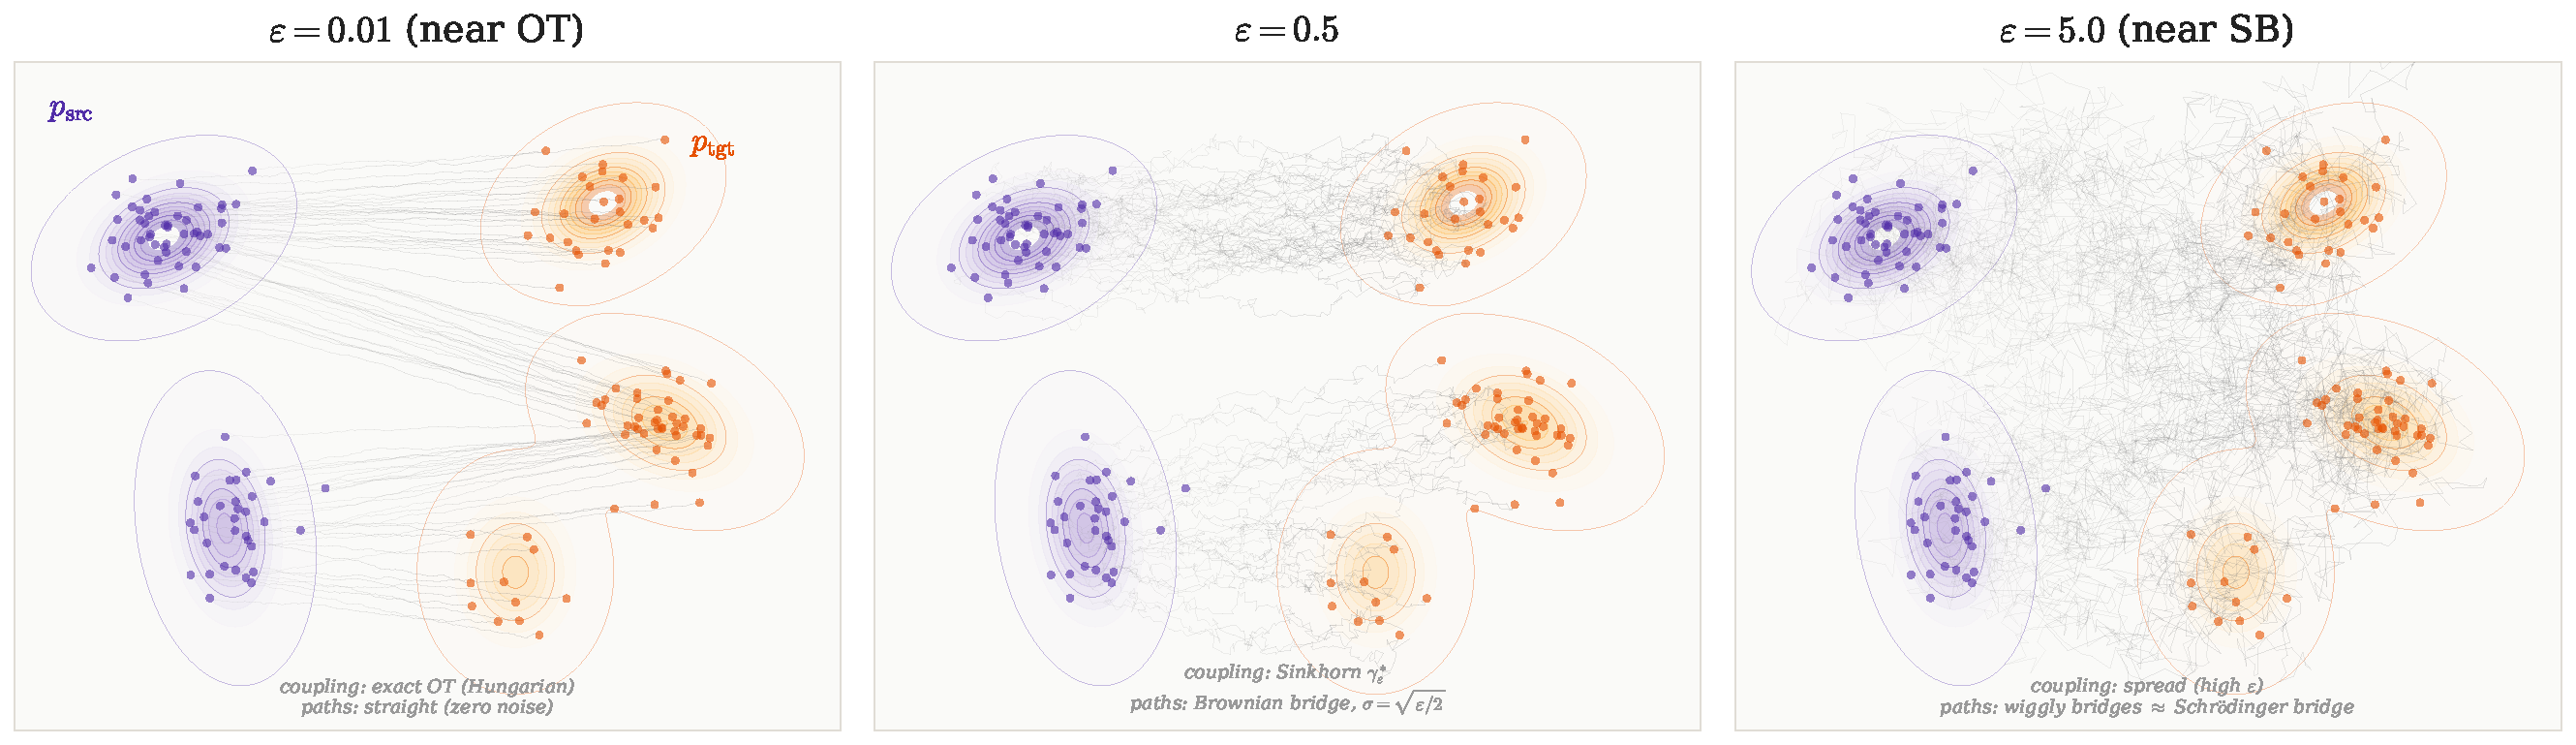
\includegraphics[width=\linewidth]{Images/PartB/eot_epsilon_interpolation.pdf}
    \caption{\textbfs{Effect of the regularization parameter $\varepsilon$ on
    entropic optimal transport (connections (iii) and (iv)).}
    As $\varepsilon$ increases, two things change simultaneously:
    the coupling $\gamma^*_\varepsilon$ spreads mass to more distant
    targets, and the transport paths become increasingly stochastic.
    Left ($\varepsilon=0.01$): paths are nearly straight and each
    source point maps to a single nearby target, recovering classical OT.
    Center ($\varepsilon=0.5$): paths acquire visible fluctuations
    and the coupling begins to spread.
    Right ($\varepsilon=2.5$): paths are highly stochastic,
    approaching the Schr\"odinger bridge regime;
    in the limit $\varepsilon\to\infty$, the coupling degenerates to
    the independent product
    $p_{\mathrm{src}}\otimes p_{\mathrm{tgt}}$.
    The couplings are computed via the Sinkhorn algorithm
    (Hungarian algorithm for $\varepsilon\to 0$);
    conditional on endpoints, the paths are Brownian bridges
    with diffusion coefficient $\sigma=\sqrt{\varepsilon/2}$
    from the Mikami duality (\Cref{subsec:sb-eot}).
    \figcredit{Created by the authors with AI-assisted coding.}}
    \label{fig:eot-epsilon}
\end{figure}

\subsection{SB and EOT are (Dual) Equivalent}\label{subsec:sb-eot}
In this section, we present two complementary perspectives showing that SB are essentially equivalent to EOT.  
Unlike classical optimal transport, which produces a single deterministic map, SB yields a \emph{stochastic} flow of particles: mass is transported probabilistically, with marginals evolving under diffusion-like dynamics.

From the static viewpoint, SB coincides with EOT, where the goal is to find a coupling between the two endpoint distributions that balances transport cost with entropy.  
From the dynamic viewpoint, SB describes a controlled diffusion process that remains as close as possible to a simple reference (such as Brownian motion) while still matching the desired endpoints.   Each perspective independently establishes the equivalence, providing two consistent ways to understand SB/EOT as canonical formulations of distribution-to-distribution transformation.



\paragraph{Static Schr\"odinger Bridge.}
Let
\[
  \widetilde R^\varepsilon(\rvx,\rvy)
  := \frac{1}{Z_\varepsilon}\,e^{-c(\rvx,\rvy)/\varepsilon}\,p_{\mathrm{src}}(\rvx)\,p_{\mathrm{tgt}}(\rvy),
\]
with normalizing constant
\[
Z_\varepsilon := \iint e^{-c(\rvx, \rvy)/\varepsilon}\, p_{\mathrm{src}}(\rvx)\, p_{\mathrm{tgt}}(\rvy)\,\mathrm d\rvx\,\mathrm d\rvy.
\]
Then, for any admissible coupling \(\gamma\in\Gamma(p_{\mathrm{src}},p_{\mathrm{tgt}})\), a direct computation gives
\[
\int c\, \mathrm d\gamma
+\varepsilon \mathcal{D}_\mathrm{KL}\!\bigl(\gamma \Vert p_{\mathrm{src}}\!\otimes\!p_{\mathrm{tgt}}\bigr)
=
\varepsilon \mathcal{D}_\mathrm{KL}\!\bigl(\gamma \Vert \widetilde R^\varepsilon\bigr)
-\varepsilon\log Z_\varepsilon.
\]
Therefore,
\begin{align}
\begin{aligned}\label{eq:eot-sb-static}
    \min_{\gamma\in\Gamma(p_{\mathrm{src}},p_{\mathrm{tgt}})}
  \Bigl\{\int c \,\mathrm d\gamma
  + \varepsilon \mathcal{D}_\mathrm{KL}\!\bigl(\gamma \Vert p_{\mathrm{src}}\!\otimes\!p_{\mathrm{tgt}}\bigr)\Bigr\}
  = \varepsilon \min_{\gamma\in\Gamma(p_{\mathrm{src}},p_{\mathrm{tgt}})}
  &\mathcal{D}_\mathrm{KL}\!\bigl(\gamma \Vert \widetilde R^\varepsilon\bigr)
  \\&-\varepsilon\log Z_\varepsilon,
\end{aligned}
\end{align}
so the entropic OT problem is equivalent, up to an additive constant, to the static Schr\"odinger Bridge problem
\[
\min_{\gamma\in\Gamma(p_{\mathrm{src}},p_{\mathrm{tgt}})}
\mathcal{D}_\mathrm{KL}(\gamma\Vert \widetilde R^\varepsilon).
\]

\paragraph{Dynamic Equivalence (Brownian Reference).} We can also understand this equivalence from a dynamical viewpoint. 
A classical result \citep{mikami2006duality} states  that entropic OT with quadratic cost
\[
c(\rvx,\rvy)=\frac{\|\rvy-\rvx\|^2}{2T}
\]
is affinely equivalent to the SB problem where the
reference path law $R^\varepsilon$ is Brownian motion on $[0,T]$,
\[
\mathrm{d}\rvx_t=\sqrt{\varepsilon}\,\mathrm{d}\rvw_t.
\]
Here, ``affinely equivalent'' means the optimal values differ by a positive scaling and an
additive constant (independent of the decision variable), so the minimizers coincide.
In particular, let $P^*$ be the optimal path distribution for SB and let $\gamma^*$ be the optimal transport plan for EOT. Then if $\rvx_{[0:T]}\sim P^*$, the pair of endpoints $(\rvx_0,\rvx_T)$ has distribution $\gamma^*$:
\[
P^* \text{ solves SB } \iff \gamma^* \text{ solves EOT and } (\rvx_0,\rvx_T)\sim\gamma^*.
\]


In words: the optimal process from the dynamic (SB) problem induces the optimal
coupling for the static (EOT) problem. Conversely, (under mild conditions on the
heat kernel,) any optimal static coupling can be realized as the endpoints of some
optimal SB process.

The key idea to derive this fact is that the KL divergence over paths can be broken down according to the endpoints, which means the Schr\"odinger bridge problem reduces to a KL divergence just over the joint distribution of $(\rvx_0,\rvx_T)$. For Brownian motion the transition density between $\rvx$ and $\rvy$ has a Gaussian form, so its negative log is quadratic:
\[
-\varepsilon\log p_T(\rvy\mid\rvx)=\frac{\|\rvy-\rvx\|^2}{2T}+\text{const}.
\]
This shows that the endpoint KL is exactly the same as the entropic OT objective with quadratic cost, up to an irrelevant constant.


\paragraph{SB with General Reference Determines the EOT Cost.}
As we discussed in \Cref{eq:sb-epsilon-general}, the SB problem is not restricted to Brownian motion; it can be defined with any (well-posed) reference process. This choice uniquely determines the cost function in the corresponding EOT problem. The key connection is that the SB \emph{reference dynamics} induce the EOT \emph{cost function}. 

Let the reference process be governed by an SDE over $[0,T]$, yielding a transition density $p_T(\rvy|\rvx)$, the likelihood of reaching $\rvy$ at time $T$ from $\rvx$ at time $0$. Then, the EOT cost function is given (up to a scaling constant) by
\[
c(\rvx, \rvy) \propto -\log p_T(\rvy|\rvx).
\]
With this cost, solving the SB problem becomes equivalent to solving an EOT problem. In short, choosing the reference dynamics in SB is mathematically equivalent to specifying the transport cost in EOT. By \Cref{eq:eot-sb-static}, the entropic OT objective differs from the static SB objective; hence the two problems are equivalent and have the same minimizer.





\subsection{EOT$_\varepsilon$ is Reduced to OT as $\varepsilon\to 0$}\label{subsec:eot-ot}


Let $\gamma^*_\varepsilon$ denote the optimal plan for the EOT$_\varepsilon$, and let $\gamma^*$ be an optimal plan for the unregularized OT problem in \Cref{eq:ot}.  The following result~\citep{mikami2008optimal, peyre2019computational} shows that as $\varepsilon \to 0$, the entropic optimal plan $\gamma^*_\varepsilon$ converges (in a suitable sense) to the OT plan $\gamma^*$, and the EOT cost converges to the OT cost. 
% \footnote{Note that even the convergence of the EOT cost to the OT cost does not hold in general, as in \citep[Example 5.1]{nutz2021introduction} with
% \begin{equation*}
%     c(\rvx,\rvy) = 
%     \begin{cases}
%         1, \ \ \rvx \neq \rvy,\\
%         0, \ \ \rvx = \rvy.
%     \end{cases}
% \end{equation*}
% \jcc{check this and elaborate this. what the main message of this: like missing some necessary conditions or what? i think we need to have some "conclusion" with footnotes as well. I agree to have counter-example but I was expecting more explanatory; otherwise, readers may be confused: we stated in the main content that the convergence hold, but suddenly we said it won't held in general.}
% }.



This convergence result is both fundamental and practically important. One of the reasons is that the entropy-regularized OT problem $\mathrm{EOT}_\varepsilon$ admits efficient numerical solutions via algorithms such as Sinkhorn. Thus, the result provides theoretical justification for using $\mathrm{EOT}_\varepsilon$ with small $\varepsilon$ as a computationally tractable proxy for the classical OT problem in \Cref{eq:ot}, even when the cost function $c(\rvx, \rvy)$ is more general than the quadratic case.


\thmp{(Informal) EOT$_\varepsilon$ Converges to OT.}{eot-ot}{
As $\varepsilon \to 0$, the optimal values converge:
\[
\lim_{\varepsilon \to 0}  \mathrm{EOT}_\varepsilon(p_{\mathrm{src}}, p_{\mathrm{tgt}}) = \mathrm{OT}(p_{\mathrm{src}}, p_{\mathrm{tgt}}). 
\]
Moreover, the optimal plans $\gamma^*_\varepsilon$ \emph{converge weakly}\ to $\gamma^*$. That is, 
\[
\mathbb{E}_{(\rvx, \rvy)\sim\gamma^*_\varepsilon}[g(\rvx, \rvy)] \to \mathbb{E}_{(\rvx, \rvy)\sim\gamma^*}[g(\rvx, \rvy)],
\]
for all bounded continuous (test) functions $g : \mathbb{R}^D \times \mathbb{R}^D \to \mathbb{R}$.
}
{For a rigorous proof, we refer to the literature~\citep{mikami2008optimal, peyre2019computational}. Below we provide a heuristic derivation of the value convergence.

Let us denote the corresponding optimal values by
\[
V_\varepsilon := \mathrm{EOT}_\varepsilon(p_{\mathrm{src}}, p_{\mathrm{tgt}}), \quad
V_0 := \mathrm{OT}(p_{\mathrm{src}}, p_{\mathrm{tgt}})
\]
for notational simplicity. 


\proofparagraph{Upper Bound.} By optimality of $\gamma^*_\varepsilon$, its value $V_\varepsilon$ is bounded by the cost of using the plan $\gamma^*$:
\[
    V_\varepsilon \leq \int c  \diff\gamma^* + \varepsilon \mathcal{D}_{\text{KL}}(\gamma^* \| p_{\mathrm{src}} \otimes p_{\mathrm{tgt}}).
\]
Assuming the KL term is a finite constant $K$, we get $V_\varepsilon \leq V_0 + \varepsilon K$. Taking the limit superior yields $\limsup_{\varepsilon \to 0} V_\varepsilon \leq V_0$.

\proofparagraph{Lower Bound.} Since the KL-divergence is non-negative, $V_\varepsilon \geq \int c  \diff\gamma^*_\varepsilon$. By definition of $V_0$ as the minimal transport cost, any plan's cost is at least $V_0$, so $\int c  \diff\gamma^*_\varepsilon \geq V_0$. This implies $V_\varepsilon \geq V_0$ for all $\varepsilon > 0$, and thus $\liminf_{\varepsilon \to 0} V_\varepsilon \geq V_0$.

Combining the upper and lower bounds shows the convergence of the optimal value, $\lim_{\varepsilon \to 0} V_\varepsilon = V_0$. The convergence of the optimal plan itself, $\gamma^*_\varepsilon \to \gamma^*$ in the weak sense, is a more advanced result from $\Gamma$-convergence theory that we omit.

 }





\subsection{SB$_\varepsilon$ is Reduced to OT as $\varepsilon\to 0$}\label{subsec:sb-ot}
For each $\varepsilon > 0$, let $\mathbf{v}_t^\varepsilon$ be a minimizer of the SB problem as in \Cref{eq:sb-epsilon-kinetic}, and let $p_t^\varepsilon$ be the marginal distribution of the controlled SDE $\mathbf{x}_t$ induced by $\mathbf{v}_t^\varepsilon$. Then $p_t^\varepsilon$ satisfies the associated Fokker–Planck equation. In contrast, denote by $(p_t^0, \mathbf{v}_t^0)$ a minimizer of the Benamou–Brenier formulation of optimal transport (see \Cref{eq:bb-ot}).

The following theorem\footnote{We remark that the convergence of the optimal values in the theorem is in the sense of \emph{$\Gamma$-convergence}, rather than a classical pointwise limit. Although this requires more technical background, we omit the details here and state only the conceptual result.} states that as $\varepsilon \to 0$, the SB problem converges to the OT problem. This result is practically important for reasons similar to those in Theorem~\ref{thm:eot-ot}. The objective $ \mathrm{SB}_\varepsilon $ can be efficiently solved using Sinkhorn type algorithms, yielding a numerically tractable and differentiable proxy for optimal transport. This is especially valuable in high dimensional or large scale settings, where direct solvers (e.g., based on the Benamou–Brenier formulation) become computationally expensive.






\thmp{(Informal) SB$_\varepsilon$ Converges to OT.}{sb-ot}{ As $\varepsilon \to 0$, we have:
\[
\lim_{\varepsilon \to 0} \text{SB}_\varepsilon(p_{\mathrm{src}}, p_{\mathrm{tgt}}) = \text{OT}(p_{\mathrm{src}}, p_{\mathrm{tgt}}),
\]
where OT is of the Benamou–Brenier formulation as in \Cref{eq:bb-ot}. Moreover, $p_t^\varepsilon $ converges weakly to  $ p_t^0$, and $\mathbf{v}_t^\varepsilon$ converges weakly to  $ \mathbf{v}_t^0$  in the appropriate function spaces.
}{A full rigorous proof of the convergence result is beyond our scope; we refer the reader to \citet{leonard2012schrodinger,leonard2014survey} for detailed derivations. Nevertheless, we can heuristically understand why this convergence may hold.

In the stochastic control formulation of the SB problem \Cref{eq:sb-epsilon-kinetic}, the controlled SDE is given by:
\[
\diff \rvx_t = \mathbf{v}_t^\varepsilon(\rvx_t)\,\diff t + \sqrt{\varepsilon}\,\diff \mathbf{w}_t.
\]
As $\varepsilon \to 0$, the noise term vanishes, and the SDE formally approaches a deterministic ODE:
\[
\diff \rvx_t = \mathbf{v}_t^0(\rvx_t)\,\diff t.
\]
This suggests that the optimal value of the SB problem converges to that of the optimal transport problem:
\[
\lim_{\varepsilon \to 0} \mathrm{SB}_\varepsilon(p_{\mathrm{src}}, p_{\mathrm{tgt}}) = \mathrm{OT}(p_{\mathrm{src}}, p_{\mathrm{tgt}}).
\]

In parallel, the marginal density $p_t^\varepsilon$ satisfies the Fokker-Planck equation:
\[
\partial_t p_t^\varepsilon + \nabla \cdot \left(p_t^\varepsilon \mathbf{v}_t^\varepsilon\right) = \frac{\varepsilon}{2}\,\Delta p_t^\varepsilon.
\]
Again, as $\varepsilon \to 0$, the diffusion term vanishes, and the equation formally reduces to the continuity equation:
\[
\partial_t p_t^0 + \nabla \cdot \left(p_t^0 \mathbf{v}_t^0\right) = 0.
\]
}

Until now, we have presented the fundamental equivalences (under their respective assumptions) between EOT and SB, as well as their important connection to OT through a limiting process, illustrated in \Cref{fig:ot-dm}. Next, we will explore how diffusion models connect to these concepts.

\newpage

\section{Is Diffusion Model's SDE Optimal Solution to SB Problem?}\label{sec:dm-and-sb}


\subsection{Diffusion models as a Special Case of Schrödinger Bridges}

SB framework extends (score-based) diffusion models by enabling nonlinear interpolation between arbitrary source and target distributions. It achieves this by adding control drift terms derived from scalar potentials $\Psi(\mathbf{x}, t)$ and $\widehat{\Psi}(\mathbf{x}, t)$, which guide a reference diffusion process to match prescribed endpoint marginals (see \Cref{eq:pde-schrodinger}) and follow the decomposition:
\[
\nabla\log{\Psi(x,t)}+\nabla\log{\hat{\Psi}(x,t)}=\nabla \log p_t^{\mathrm{SB}}(\mathbf{x}).
\]
This generalization allows the model to move beyond standard Gaussian priors and generate samples from broader distributions.

\paragraph{Connection to Diffusion Models.}

Diffusion models arise as a special case of the SB framework. Suppose the potential is constant, $\Psi(\mathbf{x}, t) \equiv 1$. Under this assumption, the second PDE in \Cref{eq:pde-schrodinger} reduces to the standard Fokker–Planck equation, whose solution is the marginal density of the reference process:
\begin{align}\label{eq:sb-backward-potential}
    \widehat{\Psi}(\mathbf{x}, t) = p_t^{\mathrm{SB}}(\mathbf{x}).
\end{align}
The corresponding SB forward SDE thus becomes the uncontrolled reference process:
\[
    \diff\mathbf{x}_t = \mathbf{f}(\mathbf{x}_t, t)\diff t + g(t)\diff\mathbf{w}_t,
\]
and the SB backward SDE simplifies to:
\[
    \diff\mathbf{x}_t = \left[\mathbf{f}(\mathbf{x}_t, t) - g^2(t) \nabla \log p_t^{\mathrm{SB}}(\mathbf{x}_t) \right]\diff t + g(t)\diff\bar{\mathbf{w}}_t,
\]
which matches Anderson’s reverse-time SDE used in diffusion models. This correspondence shows that diffusion models can be interpreted as the zero-control limit of SB, where no additional drift is introduced by the potentials.

\paragraph{Boundary Conditions and Generality.}
The above reduction is purely formal unless the boundary constraints are compatible. For arbitrary
source/target $(p_{\mathrm{src}},p_{\mathrm{tgt}})$, the PDE boundary conditions in
\Cref{eq:pde-schrodinger} are generally not satisfied by the choice $\Psi\equiv 1$.
Full SB resolves this by learning nontrivial potentials that induce a nonlinear control
drift, bending the reference dynamics to match any prescribed endpoints. By contrast,
diffusion models fix one endpoint to a simple prior (typically Gaussian) and learn only the
reverse-time score to reach the data. With this perspective, SB is the more flexible umbrella: with nontrivial
potentials it bridges arbitrary endpoints; with $\Psi\equiv 1$ it collapses to the diffusion-model
case above. We additionally remark that in the standard linear diffusion model, $p_T \approx p_{\mathrm{prior}}$ holds only as $T \to \infty$, so the match to the prior is merely approximate.



% SB framework extends (score-based) diffusion models by enabling nonlinear interpolation between arbitrary source and target distributions. It achieves this by adding control drift terms derived from scalar potentials $\Psi(\mathbf{x}, t)$ and $\widehat{\Psi}(\mathbf{x}, t)$, which guide a reference diffusion process to match prescribed endpoint marginals (see \Cref{eq:pde-schrodinger}) and follow the following decomposition:
% \[
% \nabla\log{\Psi(x,t)}+\nabla\log{\hat{\Psi}(x,t)}=\nabla \log p_t^{\mathrm{SB}}(\mathbf{x})
% \]
% This generalization allows the model to move beyond standard Gaussian priors and generate samples from broader distributions.

% \paragraph{Connection to Diffusion Models.}

% Diffusion models arise as a special case of the SB framework. Suppose the forward potential is constant, $\Psi(\mathbf{x}, t) \equiv 1$. Under this assumption, the second PDE in \Cref{eq:pde-schrodinger} reduces to the standard Fokker–Planck equation, whose solution is the marginal density of the reference process:
% \begin{align}\label{eq:sb-backward-potential}
%     \widehat{\Psi}(\mathbf{x}, t) = p_t^{\mathrm{SB}}(\mathbf{x}).
% \end{align}
% The corresponding SB forward SDE thus becomes the uncontrolled reference process:
% \[
%     \diff\mathbf{x}_t = \mathbf{f}(\mathbf{x}_t, t)\diff t + g(t)\diff\mathbf{w}_t,
% \]
% and the SB backward SDE simplifies to:
% \[
%     \diff\mathbf{x}_t = \left[\mathbf{f}(\mathbf{x}_t, t) - g^2(t) \nabla \log p_t^{\mathrm{SB}}(\mathbf{x}_t) \right]\diff t + g(t)\diff\bar{\mathbf{w}}_t,
% \]
% which matches Anderson’s reverse-time SDE used in diffusion models. This correspondence shows that diffusion models can be interpreted as the zero-control limit of SB, where no additional drift is introduced by the potentials.

% \jcc{However, if for general $p_{\mathrm{src}}$ and  $p_{\mathrm{tgt}}$, the boundary conditions of \Cref{eq:pde-schrodinger} would not be generally satisfied. SB in this PDE formulation provide a flexible and general nonlinear drift to drag to any pre-given endpoint distributions, unlike diffusion model which fixes one endpoint as a Gaussian prior.}

\subsection{Diffusion Models as Schrödinger Half-Bridges}

In this section, we explain why diffusion models are not full Schr\"odinger bridges, 
but can instead be understood through the relaxed notion of \emph{Schr\"odinger half-bridges}. 
A half-bridge enforces only one endpoint constraint (either $p_{\mathrm{prior}}$ or $p_{\mathrm{data}}$) rather than both, 
making it a one-sided variant of the full bridge. 
Before formalizing this connection, we introduce the definition of Schr\"odinger half-bridges, 
building on the general formulation in \Cref{eq:sb-epsilon-general} with arbitrary $p_{\mathrm{src}}$ and $p_{\mathrm{tgt}}$. 
We will then return to diffusion models and show how the half-bridge viewpoint naturally applies when the 
endpoints are given by $p_{\mathrm{prior}}$ and $p_{\mathrm{data}}$.



\paragraph{Schrödinger Half-Bridges}

The SB problem asks for a stochastic process whose law is
closest (in KL divergence) to a simple reference process, while \emph{matching
two endpoint distributions} $p_{\mathrm{src}}$ and $p_{\mathrm{tgt}}$.
Solving the full bridge requires enforcing both boundary conditions,
which is often computationally difficult. A useful relaxation is the
\emph{half-bridge} problem: instead of matching both endpoints, we match
only one of them. 

Formally, let $R$ be the reference path distribution. 
The \emph{forward half-bridge} seeks a path distribution $P$ minimizing
\[
    \min_{P: P_0 = p_{\mathrm{src}}}
    \mathcal{D}_{\mathrm{KL}}(P \,\|\, R),
\]
subject to the single constraint $P_0 = p_{\mathrm{src}}$. 
Similarly, the \emph{backward half-bridge} constrains only the terminal
distribution,
\[
    \min_{P: P_T = p_{\mathrm{tgt}}}
    \mathcal{D}_{\mathrm{KL}}(P \,\|\, R).
\]
In words, the forward half-bridge asks: among all processes starting
from the desired initial distribution, which one looks most like the
reference? The backward half-bridge asks the same question for processes
ending at the desired terminal distribution. By combining these two
relaxations iteratively, one can approximate the full SB.





\paragraph{Diffusion Models Miss Exact Endpoint Matching.}
A key difference between diffusion models and the SB framework lies in the treatment of the terminal distribution $p_T$. In standard diffusion models, the forward SDE is typically linear in $\rvx_t$ (see \Cref{eq:forward-linear-sde}) and designed so that $p_T$ approximates the  prior only as $T \to \infty$:
\[
    p_T \approx p_{\mathrm{prior}}.
\]
At finite time, however, $p_T$ is a Gaussian whose parameters depend on $p_{\text{data}}$ (see \Cref{subsec:rigorous-proof-linear-sde}). As a result, it generally does not match the desired prior without careful tuning.



In contrast, the SB framework enforces exact marginal matching at a finite time $T$ by introducing an additional control drift of the form $g^2(t)\nabla_\mathbf{x}\log \Psi(\mathbf{x}, t)$. This ensures that the terminal distribution precisely satisfies $p_T = p_{\mathrm{prior}}$, regardless of the initial data distribution $p_0 = p_{\mathrm{data}}$. In summary:
\begin{itemize}
    \item \textbfs{Diffusion Models:} $p_T \approx p_{\mathrm{prior}}$, asymptotically as $T \to \infty$,
    \item \textbfs{Schrödinger Bridge:} $p_T = p_{\mathrm{prior}}$ exactly at finite $T$, enabled by solving for the control potentials $\Psi$ and $\widehat{\Psi}$.
\end{itemize}

\paragraph{Diffusion Schrödinger Bridge.} 
Standard diffusion models do not enforce $P_T = p_{\mathrm{prior}}$, and thus only solve a Schrödinger \emph{half-bridge} from $p_{\mathrm{data}}$ to $p_{\mathrm{prior}}$.

To address this, the Diffusion Schrödinger Bridge (DSB)~\citep{de2021diffusion} alternates between matching both endpoint marginals by following the idea of the Iterative Proportional Fitting (IPF) algorithm, an alternating projection method. This extends diffusion models to solve the full SB problem as follows\footnote{Although this description uses $p_{\mathrm{data}}$ and $p_{\mathrm{prior}}$, the DSB framework applies to any pair of endpoint distributions.}:

\begin{itemize}
    \item \textbfs{Step 0: Reference Process.} Initialize with $P^{(0)} := R_{\text{fwd}}$, the reference forward SDE:
    \[
        \mathrm{d} \mathbf{x}_t = \mathbf{f}(\mathbf{x}_t, t)   \mathrm{d} t + g(t)   \mathrm{d} \mathbf{w}_t, \quad \mathbf{x}_0 \sim p_{\text{data}}.
    \]
    This ensures $P_0^{(0)} = p_{\text{data}}$, but typically $P_T^{(0)} \neq p_{\text{prior}}$.

    \item \textbfs{Step 1: Backward Pass.} Compute the process $P^{(1)}$ that matches $p_{\text{prior}}$ at time $T$ while staying close to $P^{(0)}$:
    \[
        P^{(1)} = \argmin_{P : P_T = p_{\text{prior}}} \mathcal{D}_{\text{KL}}(P  \|  P^{(0)}).
    \]
    This is achieved via approximating the oracle score function  with a neural network $\mathbf{s}_{\bm{\phi}^\times}$, which results in the reverse-time SDE:
    \[
        \mathrm{d} \mathbf{x}_t = \left[ \mathbf{f}(\mathbf{x}_t, t) - g^2(t) \mathbf{s}_{\bm{\phi}^\times}(\mathbf{x}_t, t) \right] \mathrm{d} t + g(t)  \mathrm{d} \bar{\mathbf{w}}_t,
    \]
    simulated backward from $\mathbf{x}_T \sim p_{\text{prior}}$.
    
    \item \textbfs{Iteration.} The process $P^{(1)}$ satisfies $P_T^{(1)} = p_{\text{prior}}$, but its initial marginal $P_0^{(1)}$ typically deviates from $p_{\text{data}}$. IPF addresses this by learning a forward SDE to adjust $P_0^{(1)}$ back to $p_{\text{data}}$, followed by another backward pass to enforce $p_{\text{prior}}$. This alternation continues, refining the process until convergence to the optimal bridge $P^*$, which satisfies both $P_0^* = p_{\text{data}}$ and $P_T^* = p_{\text{prior}}$. \citet{de2021diffusion} prove convergence under mild conditions.
\end{itemize}


The DSB formulation above is historically important and conceptually clear, but its practical implementation can be computationally demanding. The forward--backward projections are carried out iteratively, so that each IPF iteration requires solving a separate score-matching problem, while approximation errors may also accumulate across rounds. More broadly, a growing body of work seeks to alleviate these difficulties by developing Schr\"odinger bridge formulations with improved stability and scalability, and in some cases with reduced dependence on repeatedly fitting separate diffusion models throughout the iterative procedure. We do not discuss these developments in detail here, but mention them to orient interested readers to a broader literature on practical SB methods~\citep{shi2023dsbm,liu2024gsbm}.




\newpage
\section{Is Diffusion Model's ODE an Optimal Map to OT Problem?}\label{sec:pfode-ot}
In this section, we focus on quadratic-cost optimal transport problem. 




\subsection{PF-ODE Flow Is Generally Not Optimal Transport}
A natural question is whether the PF-ODE flow map coincides with the
optimal transport map under quadratic cost. The answer is no, and this
can already be seen in the simplest possible setting.
\citet{tanana2017comparison} showed that even when both the source and
target distributions are Gaussian, the PF-ODE flow map and the optimal
transport map (given by the classical closed-form Gaussian OT formula)
do not coincide. Both maps can be computed explicitly in this case, so
the non-optimality is verified by direct comparison without any heavy
machinery.

Below we present the more general construction of
\citet{lavenant2022flow}, which establishes the same conclusion for a
broader class of initial distributions and provides structural insight
into why the PF-ODE flow fails to be optimal.

\begin{figure}[th!]
    \centering
    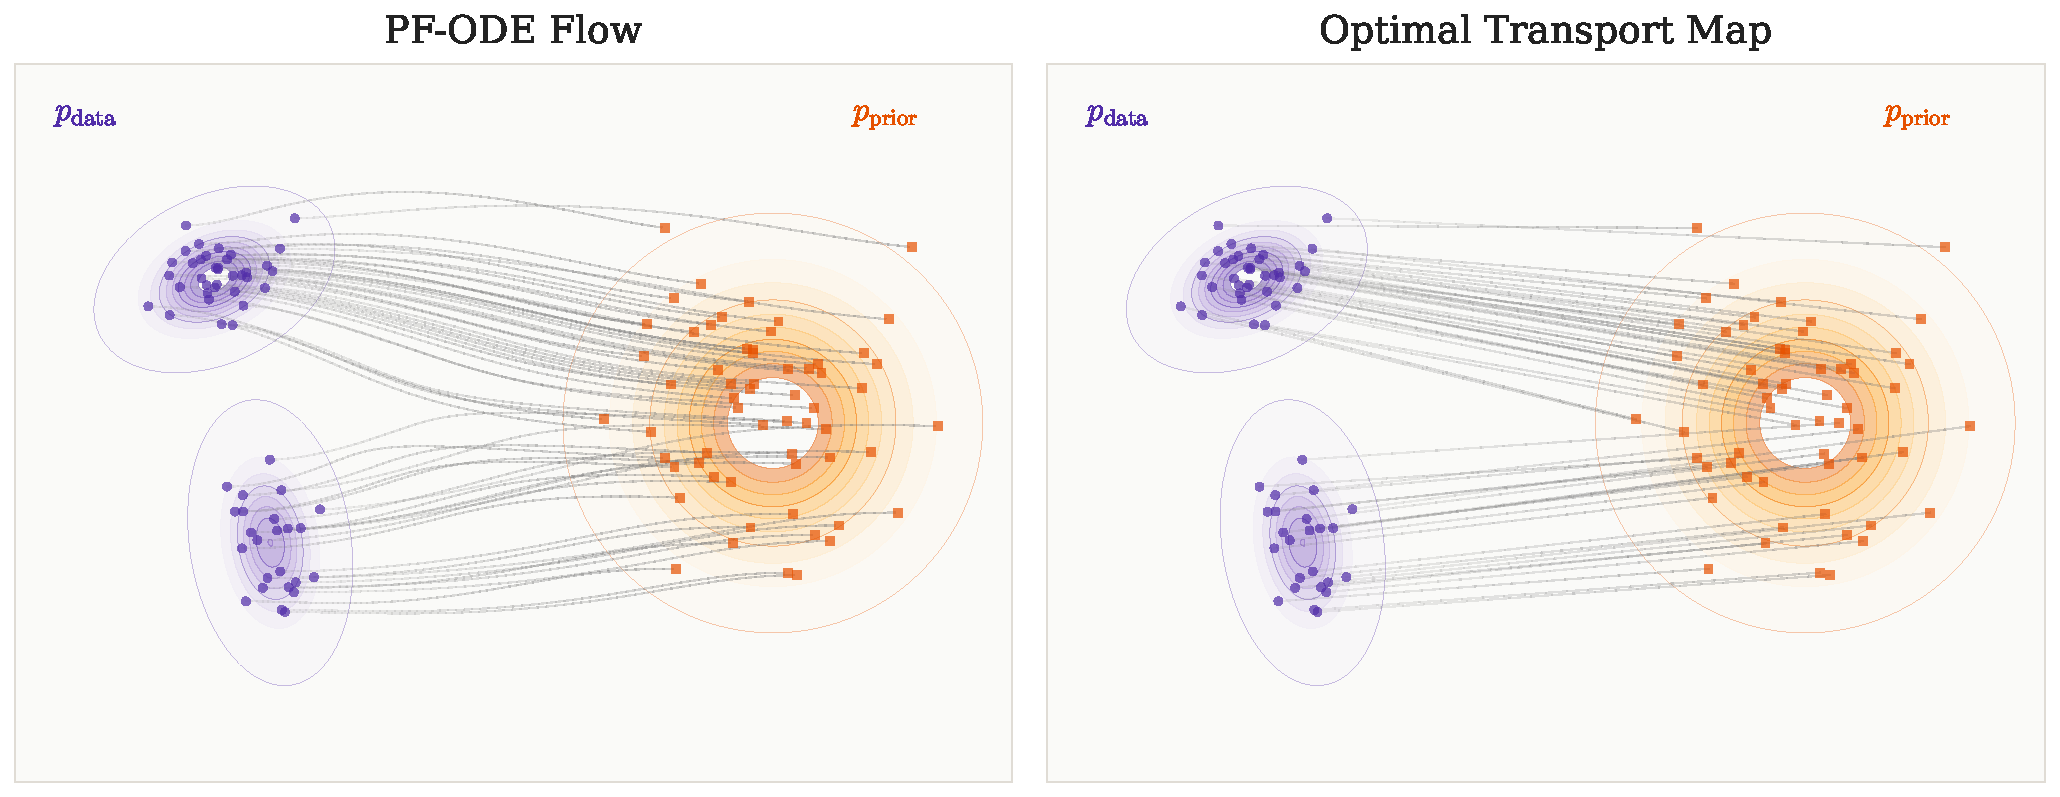
\includegraphics[width=\linewidth]{Images/PartB/pfode_vs_ot_2d.pdf}
    \caption{Comparing the PF-ODE flow map with the true OT map
    from $p_{\mathrm{data}}$ to $p_{\mathrm{prior}}$ in 2D.
    Right: the quadratic-cost OT map, computed exactly via the
    Hungarian algorithm.
    Left: the PF-ODE flow map obtained by integrating the
    PF-ODE. The two maps visibly differ,
    illustrating that the PF-ODE does not generally recover
    the optimal transport map.
    \figcredit{Created by the authors with AI-assisted coding.}}
    \label{fig:pfode-vs-ot-2d}
\end{figure}


\paragraph{Setup.} We consider a VP SDE, specifically the Ornstein–Uhlenbeck process, which evolves a smooth initial density $p_0$ toward the standard Gaussian $\mathcal{N}(\bm{0}, \rmI)$:
\[
\diff \rvx(t) = -\rvx(t) \diff t + \sqrt{2} \diff \rvw(t), \quad \rvx(0) \sim p_0.
\]
The associated PF-ODE is given by
\[
\frac{\diff \mathbf{S}_t(\rvx)}{\diff t} = -\mathbf{S}_t(\rvx) - \nabla \log p_t(\mathbf{S}_t(\rvx)), \quad \mathbf{S}_0(\rvx) = \rvx.
\]
Here, $\mathbf{S}_t$ denotes the flow map pushing forward $p_0$ to the marginal $p_t$:
\[
\left(\mathbf{S}_t\right) \# p_0 = p_t,
\quad\text{that is,}\quad
p_t(\rvy) = \int_{\mathbb{R}^D} \delta(\rvy - \mathbf{S}_t(\rvx))   p_0(\rvx) \diff \rvx.
\]
These densities $p_t$ evolve via the Fokker-Planck equation:
\[
\frac{\partial p_t}{\partial t} = \nabla \cdot (\rvx p_t) + \Delta p_t.
\]
This is equivalent to a continuity equation with velocity field:
\[
\rvv_t(\rvx) = -\rvx - \nabla \log p_t(\rvx),
\]
whose flow is given by $\mathbf{S}_t(\rvx)$. In other words, the PF-ODE can be written as: 
\[
\frac{\diff \mathbf{S}_t(\rvx)}{\diff t} = \rvv_t\left(\mathbf{S}_t(\rvx)\right).
\]

As $t \to \infty$, the map transports the initial distribution to the prior:
\[
\mathbf{S}_\infty \# p_0 = \mathcal{N}(\bm{0}, \rmI) =: p_{\text{prior}}.
\]
\paragraph{Objective of \citet{lavenant2022flow}'s Argument.}

\citet{lavenant2022flow} do not directly assess whether the terminal map $\mathbf{S}_\infty$ from $p_0$ to the Gaussian is optimal. Instead, they construct a specific initial distribution $p_0$ and examine the entire PF-ODE trajectory. Their key observation is that optimality may fail at some point along the flow.

They consider the intermediate marginal $p_t = \mathbf{S}_t \# p_0$ and define the residual transport map from $p_{t_0}$ to the Gaussian as
\[
\mathbf{T}_{t \to \infty} := \mathbf{S}_\infty \circ \mathbf{S}_{t}^{-1}, \quad \text{for all } t\geq 0.
\]
The core of their argument shows that, for a carefully chosen $p_0$, there exists a time $t_0 \geq 0$ such that $\mathbf{T}_{t_0 \to \infty}$ is not the quadratic-cost optimal transport map  from the new starting distribution $p_{t_0}$ to $\mathcal{N}(\bm{0}, \rmI)$.

This result demonstrates that PF-ODE flows do not, in general, yield optimal transport maps, and that the property of optimality can break down for certain initial distributions.

\paragraph{Some Tools.} The argument of \citet{lavenant2022flow} crucially relies on the following result, known as \emph{Brenier's theorem}:
\begin{quote}
    \begin{theorem}[Informal Brenier's Theorem]\label{thm:brenier}
Let $\nu_1, \nu_2$ be two probability distributions on $\mathbb{R}^D$ with smooth densities. A smooth map $\rmT : \mathbb{R}^D \to \mathbb{R}^D$ is the optimal transport from $\nu_1$ to $\nu_2$ (under quadratic cost) if and only if $\rmT = \nabla u$ for some convex function $u$. In this case, $\mathrm{D} \rmT$ is symmetric and positive semi-definite, and $u$ satisfies the Monge–Ampère equation:
\[
\det \mathrm{D}^2 u(\mathbf{x}) = \frac{\nu_1(\mathbf{x})}{\nu_2(\nabla u(\mathbf{x}))}.
\]
\end{theorem}
\end{quote}

The proof also implicitly uses the following fact, which we will not repeat each time: \emph{a map is the optimal transport between two distributions if and only if its inverse is the optimal transport in the reverse direction}.





\paragraph{Proof Sketch: PF-ODE Is Not an OT Map in General.} \citet{lavenant2022flow} employ a proof by contradiction: they assume that for every $t\ge0$, the map
\[
\mathbf{T}_t  =  \mathbf{S}_t \circ \mathbf{S}_\infty^{-1}
\]
is the quadratic-cost optimal transport map from $\mathcal{N}(\bm{0},\rmI)$ to $p_t$. 




\subparagraph{Step 1:  Brenier's Theorem.}  By Brenier’s Theorem, the Jacobian of any optimal transport map from Gaussian must be symmetric and positive semi-definite. Thus, 
\[
\mathrm{D} \mathbf{T}_t(\rvx) = \mathrm{D} \mathbf{S}_t(\mathbf{S}_\infty^{-1}(\rvx)) \mathrm{D} (\mathbf{S}_\infty^{-1})(\rvx)
\]
must be symmetric for all $t$ and $\rvx$. Here, $\mathrm{D} \mathbf{T}_t(\rvx)$ denotes the total differentiation with respect to $\rvx$.
\subparagraph{Step 2: Time-Differentiating the Symmetry Condition.}  
Differentiating in time:
\[
\frac{\partial}{\partial t} \mathrm{D}\mathbf{T}_t(\rvx)
= \left( \frac{\partial}{\partial t} \mathrm{D} \mathbf{S}_t \right)(\mathbf{S}_\infty^{-1}(\rvx)) \mathrm{D} (\mathbf{S}_\infty^{-1})(\rvx).
\]
Given that the symmetry holds for all $t$, it follows that this derivative remains symmetric.

Using the flow ODE (differentiating in $\rvx$), we obtain:
\[
\frac{\partial (\mathrm{D}\mathbf{S}_t)}{\partial t}
= \mathrm{D}\rvv_t(\mathbf{S}_t) \cdot \mathrm{D}\mathbf{S}_t
= \left( -\rmI - \mathrm{D}^2 \log p_t(\mathbf{S}_t) \right) \cdot \mathrm{D}\mathbf{S}_t.
\]
Combining the above, we see that
\[
\left( -\rmI - \mathrm{D}^2 \log p_t(\mathbf{S}_t) \right) \cdot\mathrm{D}\mathbf{S}_t \cdot \mathrm{D} (\mathbf{S}_\infty^{-1})
\]
is symmetric for all $t\geq 0$.

At $t = 0$, we have $\mathbf{S}_0 = \rmI$ and $\mathrm{D}\mathbf{S}_0 = \rmI$, yielding:
\[
\left( -\rmI - \mathrm{D}^2 \log p_0(\mathbf{S}_\infty^{-1}(\rvx)) \right) \cdot \mathrm{D} (\mathbf{S}_\infty^{-1})(\rvx) \quad \text{is symmetric}.
\]

\subparagraph{Step 3: The Commutation Condition.}  Since $\mathbf{T}_0 = \mathbf{S}_\infty^{-1}$ is assumed to be optimal, its Jacobian $D\mathbf{T}_0 = \mathrm{D}(\mathbf{S}_\infty^{-1})$ is symmetric.  Moreover, the Hessian $\mathrm{D}^2\log p_0$ is symmetric.  Recall that two symmetric matrices multiply to a symmetric matrix if and only if they commute.  Hence, for all $\mathbf{x}\in\mathbb{R}^D$,
\[
\mathrm{D}^2\log p_0\bigl(\mathbf{S}_\infty^{-1}(\mathbf{x})\bigr)
\quad\text{must commute with}\quad
\mathrm{D}(\mathbf{S}_\infty^{-1})(\mathbf{x}) .
\]
Setting $\mathbf{y}=\mathbf{S}_\infty^{-1}(\mathbf{x})$ gives the equivalent condition: for all $\rvy\in\mathbb{R}^D$,
\[
\mathrm{D}^2\log p_0(\mathbf{y})
\quad\text{must commute with}\quad
\mathrm{D}\mathbf{S}_\infty(\mathbf{y}) .
\]


Now, we transform this condition into a more computable form.  
Since $\mathbf{S}_\infty$ is optimal between $p_0$ and $\mathcal{N}(\bm{0},\rmI)$, Brenier’s theorem guarantees that $\mathbf{S}_\infty = \nabla u$ for some convex function $u$.  From the Monge–Ampère equation, it follows that:
\[
\log p_0(\rvy) = \log \det(\mathrm{D}^2 u(\rvy)) - \frac{1}{2} \|\nabla u(\rvy)\|^2 + \text{Constant}.
\]
The condition becomes (with $\mathrm{D}\rmS_\infty = \mathrm{D}^2 u$): 
\begin{mdframed}
\begin{align}\label{eq:necessary-ot}
\mathrm{D}^2 \left(\log \det \mathrm{D}^2 u - \frac{1}{2} \|\nabla u\|^2\right)
\quad\text{must commute with}\quad
\mathrm{D}^2 u.
\end{align}
\end{mdframed}
This yields a necessary condition for $\mathbf{T}_t$ to be optimal.
\subparagraph{Step 4: Constructing the Counterexample.} Let us show how to leverage this necessary condition to derive a contradiction.

Assume we can construct a convex function $u$ such that  
\[
\mathrm{D}^2 \left( \log \det \mathrm{D}^2 u(\mathbf{x}) - \frac{1}{2} \lvert \nabla u(\mathbf{x}) \rvert^2 \right)
\]
does not commute with $\mathrm{D}^2 u(\mathbf{x})$ for some $\mathbf{x} \in \mathbb{R}^D$.  Defining $p_0 = (\nabla u)^{-1} \# \mathcal{N}(\bm{0}, \rmI)$, Brenier's theorem implies that $\nabla u$ is the optimal transport from $p_0$ to $\mathcal{N}(\bm{0}, \rmI)$. However, the condition in \Cref{eq:necessary-ot} fails, leading to a contradiction. Thus, our goal is to construct such a function. 
Consider  
\[
u(\mathbf{x}) = \frac{1}{2} \|\mathbf{x}\|^2 + \varepsilon \phi(\mathbf{x}), \quad \text{for a small } \varepsilon.
\]
Then $\mathrm{D}^2 u(\mathbf{0}) = \rmI + \varepsilon \mathrm{D}^2 \phi(\mathbf{0})$, and the commutation condition at $\mathbf{x} = \mathbf{0}$ requires $\mathrm{D}^2 \phi(\mathbf{0})$ to commute with $\mathrm{D}^2 (\Delta \phi)(\mathbf{0})$. 

For example, in $\mathbb{R}^2$, choosing  
\[
\phi(x_1, x_2) = x_1 x_2 + x_1^4
\]
provides a counterexample where the Hessian $\mathrm{D}^2 \log p_0$ and the Jacobian $\mathrm{D}^2 u$ do not commute.

This contradiction shows that $\mathbf{T}_t$ cannot be optimal for all $t \geq 0$. Therefore, there exists some $t_0 \geq 0$ such that the map $\mathbf{T}_{t_0 \to \infty}$ is not optimal.

\newpage

\subsection{Can Canonical Linear Flow and Reflow Leads to an OT Map?}\label{subsec:ot-linear-reflow} 
We have seen that the PF-ODE (especially in VP type forward kernel) is generally not an OT map. One natural question now is:
\begin{question}
Does the linear interpolation flow $(1-t)\rvx_0 + t \rvx_1$ with $\rvx_0\sim p_{\mathrm{src}}$ and $\rvx_1\sim p_{\mathrm{tgt}}$, when applied to the independent coupling $\pi(\rvx_0, \rvx_1) = p_{\mathrm{src}}(\rvx_0)p_{\mathrm{tgt}}(\rvx_1)$, recover the OT map?
\end{question}
The answer to the question is no.
 
Nevertheless, combining a linear path with a given coupling offers a practical upper bound on the true OT cost.  Among all possible paths, linear interpolation provides the tightest such upper bound, as we will see in the following discussion.


\paragraph{Canonical Linear Flow and Optimal Transport.}
Focusing on optimal transport with quadratic cost, we consider the equivalent form of \Cref{eq:ot}, the Benamou--Brenier formulation in \Cref{eq:bb-ot}:
\begin{equation*}
    \mathcal{K}\left(p_{\mathrm{src}}, p_{\mathrm{tgt}}\right) :=  \min_{\substack{ (p_t, \rvv_t) \text{ s.t. }
        \partial_t p_t + \nabla \cdot (p_t \rvv_t) = 0, \\
        p_0 = p_{\mathrm{src}},\,\, p_1 = p_{\mathrm{tgt}}
    }}
    \int_0^1 \int_{\mathbb{R}^D} \|\rvv_t(\rvx)\|^2 p_t(\rvx) \diff\rvx \diff t.
\end{equation*}
Unlike the static Monge formulation (\Cref{eq: Monge's Formulation}),
where computing the optimal map requires solving the Monge--Amp\`ere
equation (\Cref{eq:monge-ampere}), the Benamou--Brenier problem admits a
convex reformulation after introducing the momentum field
$\rvm_t := p_t \rvv_t$. Nevertheless, discretizing this convex problem
on a grid in $\mathbb{R}^D$ remains intractable in high dimensions.




While solving the Benamou-Brenier formulation is generally intractable,  \citet{liu2022rectified,lipman2024flow} reveal that its kinetic energy admits a practical upper bound. This is achieved by restricting the search to a simpler family of \emph{conditional flows}, where each path is defined by its fixed endpoints $(\rvx_0, \rvx_1)$ drawn from a coupling $\pi_{0,1}$ of the source and target distributions. Within this \emph{conditional flow} family, the canonical linear interpolation emerges as the optimal choice, as formalized below.

\proppp{An Upper Bound on OT Kinetic Energy via Conditional Flows}{ot-conditional-flow}{
Let $\pi_{0,1}$ be any coupling between $p_{\mathrm{src}}$ and $p_{\mathrm{tgt}}$.
\begin{enumerate}
    \item[(1)] The kinetic energy is bounded above by the expected path energy of any conditional flow $\bm{\Psi}_t(\rvx_0, \rvx_1)$ that connects the endpoints:
    \begin{equation*}
        \mathcal{K}\left(p_{\mathrm{src}}, p_{\mathrm{tgt}}\right) \le \mathbb{E}_{(\rvx_0, \rvx_1) \sim \pi_{0,1}} \left[ \int_0^1 \|\bm{\Psi}'_t(\rvx_0, \rvx_1)\|^2 \diff t \right].
    \end{equation*}
    \item[(2)] The unique conditional flow $\bm{\Psi}^*_t$ that minimizes the upper bound on the right-hand side is the linear interpolation path:
    \begin{equation*}
        \bm{\Psi}^*_t(\rvx_0, \rvx_1) = (1 - t) \rvx_0 + t \rvx_1.
    \end{equation*}
  Substituting this optimal path yields the tightest version of the bound:
    \begin{equation*}
        \mathcal{K}\left(p_{\mathrm{src}}, p_{\mathrm{tgt}}\right) \le \mathbb{E}_{(\rvx_0, \rvx_1) \sim \pi_{0,1}} \|\rvx_1 - \rvx_0\|^2.
    \end{equation*}
\end{enumerate}
}{The proof relies on a straightforward application of Jensen's inequality and the tower property of conditional expectations, before solving the simplified variational problem with the Euler-Lagrange equation; we refer to \citep{lipman2024flow}'s Section 4.7 for the complete argument.}

In other words, the linear interpolation $\bm{\Psi}^*_t$ (i.e., the forward kernel used by Flow Matching and Rectified Flow) minimizes an upper bound on the true kinetic energy for any chosen coupling $\pi_{0,1}$.

We emphasize that optimality within this class of conditional flows does not guarantee global optimality on the marginal distributions. 




\paragraph{Reflow and Optimal Transport.} 
The most naive transport plan between two distributions is to connect their samples with straight lines using a simple independent coupling. However, this approach is demonstrably not optimal, as the failure lies not in the straight-line paths themselves, but in the inefficient initial pairing of points. 

The Reflow procedure may offer a constructive response. It is an iterative algorithm designed specifically to correct this pairing, and crucially, each step is guaranteed to be cost-non-increasing \citep{liu2022flow}. This property suggests Reflow systematically pushes the transport plan towards a more optimal configuration, which naturally motivates the central question of its convergence.
\begin{question}
    What happens if we apply the \texttt{Rectify} operator iteratively? Can the resulting sequence of transport plans converge to the optimal one, or does the fixed point of the Reflow process yield the OT map?
\end{question}
The short answer is no in general. Below, we explain what may go wrong. To recall, the Reflow procedure iteratively refines the coupling between $p_{\mathrm{src}}$ and $p_{\mathrm{tgt}}$ via the update:
\[
\pi^{(k+1)} = \texttt{Rectify}(\pi^{(k)}),
\]
initialized with the product coupling $\pi^{(0)} := p_{\mathrm{src}}(\rvx_0) p_{\mathrm{tgt}}(\rvx_1)$. More precisely, $\texttt{Rectify}$ output the updated coupling $\pi^{(k+1)}$ via the following: At each iteration $k = 0, 1, 2, \ldots$, a velocity field $\rvv_t^{(k)}$ is learned via:
\[
\rvv_t^{(k)} \in \argmin_{\rvu_t} \, \mathcal{L}(\rvu_t\big\vert\pi^{(k)}),
\]
where $\mathcal{L}(\rvu_t\big\vert\pi^{(k)})$ is the loss (e.g., RF or FM loss) defined in \Cref{eq:reflow-loss}. Here, for notational simplicity, we adopt a non-parametric formulation for the velocity field, rather than a parameterized form $\bm{\phi}$ employed in other contexts.
The updated coupling is then given by:
\[
\pi^{(k+1)}(\rvx_0, \rvx_1) := p_{\mathrm{src}}(\rvx_0)\, \delta\big(\rvx_1 - \bm{\Psi}_1^{(k)}(\rvx_0)\big),
\]
where $\bm{\Psi}_1^{(k)}$ denotes the solution map at time $t=1$ obtained by integrating $\rvv_t^{(k)}$ from initial condition $\rvx_0$.

It has been observed in \citep{liu2022flow} that for a coupling $\pi$ between $p_{\mathrm{src}}$ and $p_{\mathrm{tgt}}$, the existence of a velocity field $\rvv_t$ that minimizes the Reflow loss, that is, satisfies $\mathcal{L}(\rvv_t |\pi) = 0$, does not necessarily imply that the transport is optimal. 



Motivated by the Benamou–Brenier framework, where the optimal transport velocity is known to be the gradient of a potential function, \citet{liu2022rectified} proposed an additional constraint: the velocity field $\rvv_t$ should be a potential field. Accordingly, the objective in \Cref{eq:reflow-loss} is modified to restrict $\rvv_t$ to the space of gradient vector fields, also known as potential flows:
\begin{align}\label{eq:reflow-loss-gradient}
    \rvw_t^{(k)} \in \argmin_{\substack{\rvu_t:\, \rvu_t=\nabla\varphi \\ \text{for some }\varphi\colon\mathbb{R}^D\to\mathbb{R}}} \, \mathcal{L}(\rvu_t\big\vert\pi^{(k)}),
\end{align}
with the rest of the procedure remaining the same as in \texttt{Rectify}.
We denote this associated operator as $\texttt{Rectify}_{\perp}$, emphasizing the projection onto irrotational vector fields. 

Let $\pi$ be a coupling between $p_{\mathrm{src}}$ and $p_{\mathrm{tgt}}$. \citet{liu2022flow} conjecture the following equivalence characterizing optimality:
\begin{enumerate}[label=(\textit{\roman*})]
  \item $\pi$ \textit{is an optimal transport coupling.}
  \item $\pi$ \textit{is a fixed point of the potential rectification operator:}
  \[
    \pi = \texttt{Rectify}_{\perp}(\pi).
  \]
  \item \textit{There exists a gradient velocity field $\rvv_t = \nabla \varphi_t$ such that the rectify loss vanishes:}
  \[
    \mathcal{L}(\rvv_t |\pi) = 0.
  \]
\end{enumerate}
However, \citet{hertrich2025relation} exhibit two types of counterexamples:
\begin{enumerate}
  \item When the intermediate distributions $p_t$ have disconnected support, one can find fixed points of $\texttt{Rectify}_{\perp}$ with zero Reflow loss and gradient velocity fields that nonetheless fail to produce the optimal coupling.
  \item Even when both endpoint distributions are Gaussian, there exist couplings whose loss is arbitrarily small but whose deviation from the optimal coupling is arbitrarily large.
\end{enumerate}

Therefore, while rectified flows may yield strong generative models, their reliability as optimal transport solvers remains limited. This highlights an important gap between generative modeling and principled optimal transport theory, inviting further research at their intersection.

Finally, we note that transport cost does not always correlate with downstream performance; as such, computing the exact optimal transport map may not necessarily lead to better practical outcomes. Nonetheless, variants of optimal transport remain fundamental to many problems in science and engineering. Diffusion models offer a powerful framework for exploring these challenges.

\newpage
\section{Closing Remarks}
In this chapter, we revisited the classical problem of transporting one
distribution to another through the lens of optimal transport and its
entropic variants. We reviewed optimal transport in both its static
Monge--Kantorovich form and its dynamic Benamou--Brenier formulation,
where transport is realized by a deterministic flow minimizing kinetic
cost. We then discussed entropy-regularized optimal transport and the
Schr\"odinger bridge (SB), which replace deterministic transport by the
most likely controlled diffusion relative to a reference process. From
this perspective, diffusion models lie naturally near the SB viewpoint
on the stochastic side, while their PF-ODEs define deterministic
transport maps on the ODE side. As we emphasized, however, the PF-ODE
transport is generally \emph{not} the quadratic-cost optimal transport
map: it is one deterministic coupling among many, rather than the
minimizer of the Benamou--Brenier action.

This also highlights a more basic question: before asking whether a
transport is optimal, \emph{when can two distributions be connected by a
deterministic map at all?} In many settings, existence is not the main
difficulty. Under mild regularity assumptions, one can often find a
measurable map $\rmT$ such that
$\rmT_\# p_{\mathrm{src}} = p_{\mathrm{tgt}}$. The harder issue is that,
beyond one dimension, relatively few classical constructions are both
explicit and robust in practice. In one dimension, the monotone
rearrangement gives a simple answer by matching quantiles. In higher
dimensions, several important constructions are known: Brenier's theorem
(Theorem~\ref{thm:brenier}) yields the quadratic-cost optimal map under
suitable regularity; the Knothe--Rosenblatt
rearrangement~\citep{rosenblatt1952remarks,knothe1957contributions}
builds a triangular map from iterated conditional distributions; and the
Dacorogna--Moser approach~\citep{dacorogna1990partial} constructs smooth
diffeomorphic transports through a velocity field solving a divergence
equation. Each gives a principled route to deterministic transport, but
each also relies on structural assumptions or nontrivial analytical
machinery.

From this viewpoint, diffusion-based flow maps provide an appealing and
flexible alternative. Rather than prescribing a closed-form transport
map, diffusion models and flow-matching methods learn a time-dependent
vector field whose induced flow pushes a simple source distribution
toward the target. This learned map need not coincide with the Brenier
map or any other classical canonical construction, and in general it
does not solve a prescribed optimal transport problem. Nevertheless, it
offers a practical and expressive route to map-based sampling in high
dimensions, where explicit transport-map constructions are often
unavailable or difficult to compute. In this sense, diffusion flows are
best understood not as replacements for classical transport theory, but
as modern learned transport mechanisms that sit alongside optimal
transport maps, triangular rearrangements, and PDE-based constructions
within the broader landscape of deterministic transport.
\newpage

